\chapter{Evaluation} \label{chp:Evaluation}
In this chapter we want to present and discuss our evaluation results. Using Baselines Lab, we perform tests in a variety of different scenarios. After explaining our general test procedure in Section \ref{sec:TestProcedure}, we will begin, by evaluating the basic components for solving maze environments. In Section \ref{sec:EvalReward} we will take a look at reward generation and continue with a deeper look into observation generation and preprocessing in Section \ref{sec:EvalObs}. Section \ref{sec:EvalRLAlgorithms} will shine some light on the question which learning algorithm performs best when dealing with our particle navigation task and we will wrap up the evaluation of the basic parameters in Section \ref{sec:EvalParameters} where we take a look at the influence of various RL hyperparameters.

The initial tests will allow us to generate a baseline for the performance of our model, which then will be used throughout the rest of the evaluation to compare the influence of other factors. We begin, by testing how much inaccuracy in both actions and observations will influence the agent in Section \ref{sec:EvalError} and continue with the extension of the particle model with physical particles in Section \ref{sec:EvalPhysical}. We will then take a look at randomized instances in Section \ref{sec:EvalRandomness} and finish with a comparison with algorithmic approaches in Section \ref{sec:EvalAlgorithms}.


\section{Test Procedure} \label{sec:TestProcedure}
In this section we want to talk about different aspects of our test procedure.

\paragraph{Environment.}
All experiments were done on a Linux workstation running Ubuntu 18.04 LTS. The workstation has an Intel 6700K CPU, a single Nvidia GeForce GTX 1080 Ti GPU and 64GB of main memory. We installed Python 3.7.3 using the Anaconda \cite{anaconda} software distribution. We also used Tensorflow 1.14 in conjunction with the CUDA Toolkit version 10.1.243 and CUDNN version 7.6.5. Baselines Lab was developed on top of Stable-Baselines 2.10 and NumPy 1.17. For a complete list of installed packages see Appendix \ref{apx:BaselinesLab}.

\paragraph{Procedure.}
Our experiments involved several sources of randomness. To ensure consistent executions, we fixed the random seed for all involved components to the same value for all experiments. Unfortunately Tensorflow 1.14 does not guarantee consistent results during GPU computations. We therefore repeated experiments three times and averaged the results for comparison. The learning curves provided in this chapter are also smoothed by an exponential weighted moving average, using a factor of $0.6$.

To determine the performance of a configuration, we look at the end result during training for the average and best trial. We also determine the step in which the average episode length becomes smaller by five percent in comparison to the environments' time limit. We call this moment the \textit{drop}, since performance usually suddenly increases when the agent is able to reach the goal for the first time. The drop can be used as an indicator for how fast the agent is able to find a first usable result, while the end-of-training episode length is an indicator for how good the best solution is the agent is able to find. 

\paragraph{Initial Hyperparameters.}
For our initial experiments we wanted to use general purpose hyperparameters for the PPO algorithm. We therefore used parameters similar to the parameters used in the RND paper \cite{burda2018exploration} (see Table \ref{tab:PPOHyperparemeters}) which showed to produce good results across all Atari environments. 


\begin{table} [ht]
    \begin{center}
        \begin{tabular}{|c|c|}
            \hline
            Hyperparameter & Value \\
            \hline
            Rollout Length & 256 \\
            Number of minibatches & 8 \\
            Number of optimization epochs & 16 \\
            Number of parallel environments & 64 \\
            Learning rate & 0.0001 \\
            Optimization algorithm & Adam \cite{kingma2014adam} \\
            $\lambda$ & 0.95 \\
            Entropy coefficient & 0.001 \\
            $\gamma$ & 0.99 \\
            Clip range & [0.9, 1.1] \\
            \hline
        \end{tabular}
    \end{center}
    \caption[Default Hyperparameters]{Default hyperparameters for PPO for the initial experiments.} \label{tab:PPOHyperparemeters}
\end{table}

We also used a common preprocessing pipeline for the observations which was also used in previous experiments \cite{huang2019}:

\begin{table} [h]
    \begin{center}
        \begin{tabular}{|c|c|}
            \hline
            Hyperparameter & Value \\
            \hline
            Observation downsampling & (84, 84) \\
            Max steps per episode & 2000 \\
            Max and skip Frames & 4 \\
            Frame stacking & 4 \\
            \hline
        \end{tabular}
    \end{center}
    \caption[Default Observation Preprocessing]{Default observation preprocessing for all environments.} \label{tab:RNDPreprocessing}
\end{table}

If not stated otherwise, we also normalized the observations by $x \mapsto x/255$. Observations for the RND curiosity module are normalized by $x \mapsto CLIP((x-\mu)/\sigma, [-5, 5])$ instead and no frame stacking is applied.


\paragraph{Instances.}
To allow easy comparison, we used the same instances as in previous work for our experiments. We included a description of these instances in Table \ref{tab:TestInstances}. Previous work showed, that these instances provide a good scale of difficulty between easy (\texttt{Corridor}) and hard (\texttt{Brain}). Instances with less paths to the goal position seem to be harder to solve, since they require more precise manoeuvering instead of just pulling all particles into a general direction. To increase the difficulty of our medium instance, we replaced it with an instance generated by our RRT instance generator. This instance can also be seen in Table \ref{tab:TestInstances} and is called \texttt{Vessel}. The Vessel maze has similar dimensions in comparison with Corridor, but has far more fine grained structures where particles may get stuck. There is also only a single path to the goal position. Additionally the Vessel maze only has a small percentage of blocked pixels, allowing for a lot more possible states than Corridor. 

\begin{table} [h!]
    \begin{center}
        \begin{tabular}{cccccc}
            \toprule
            Instance & Name & Dimension & Size (\% of Area) & $d_{avg}$ & $d_{max}$ \\
            \midrule
            
            \parbox[c]{3.5cm}{
\includegraphics[clip, width=3.5cm]{figures/evaluation/procedure/corridor_upscaled.png}} & Corridor & $(100 \times 100)$ & $2869 \ (= 28.69\%)$ & 73.65 & 117 \\
            \addlinespace[0.05cm]
            \midrule
            
            \parbox[c]{3.5cm}{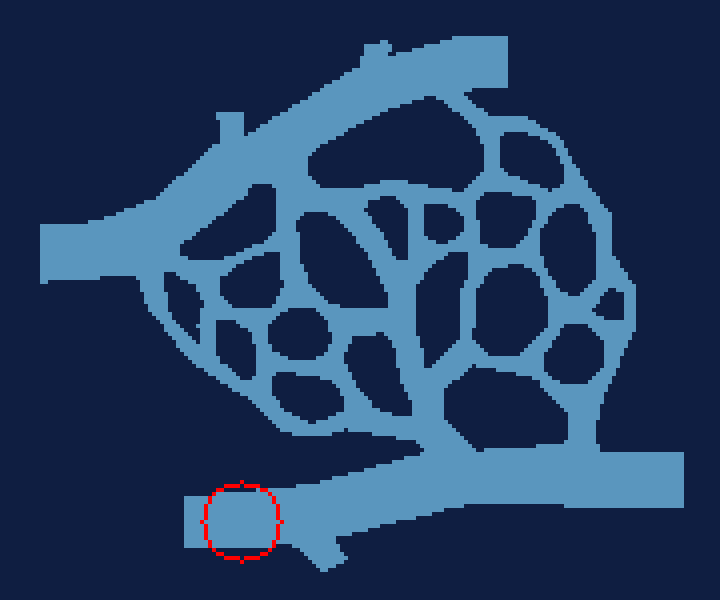
\includegraphics[clip, width=3.5cm]{figures/evaluation/procedure/capillary_upscaled.png}} & Capillary & $(180 \times 150)$ & $7169 \ (\approx 26.55\%)$ & 91.22 & 149 \\
            \addlinespace[0.05cm]
            \midrule
            
            \parbox[c]{3.5cm}{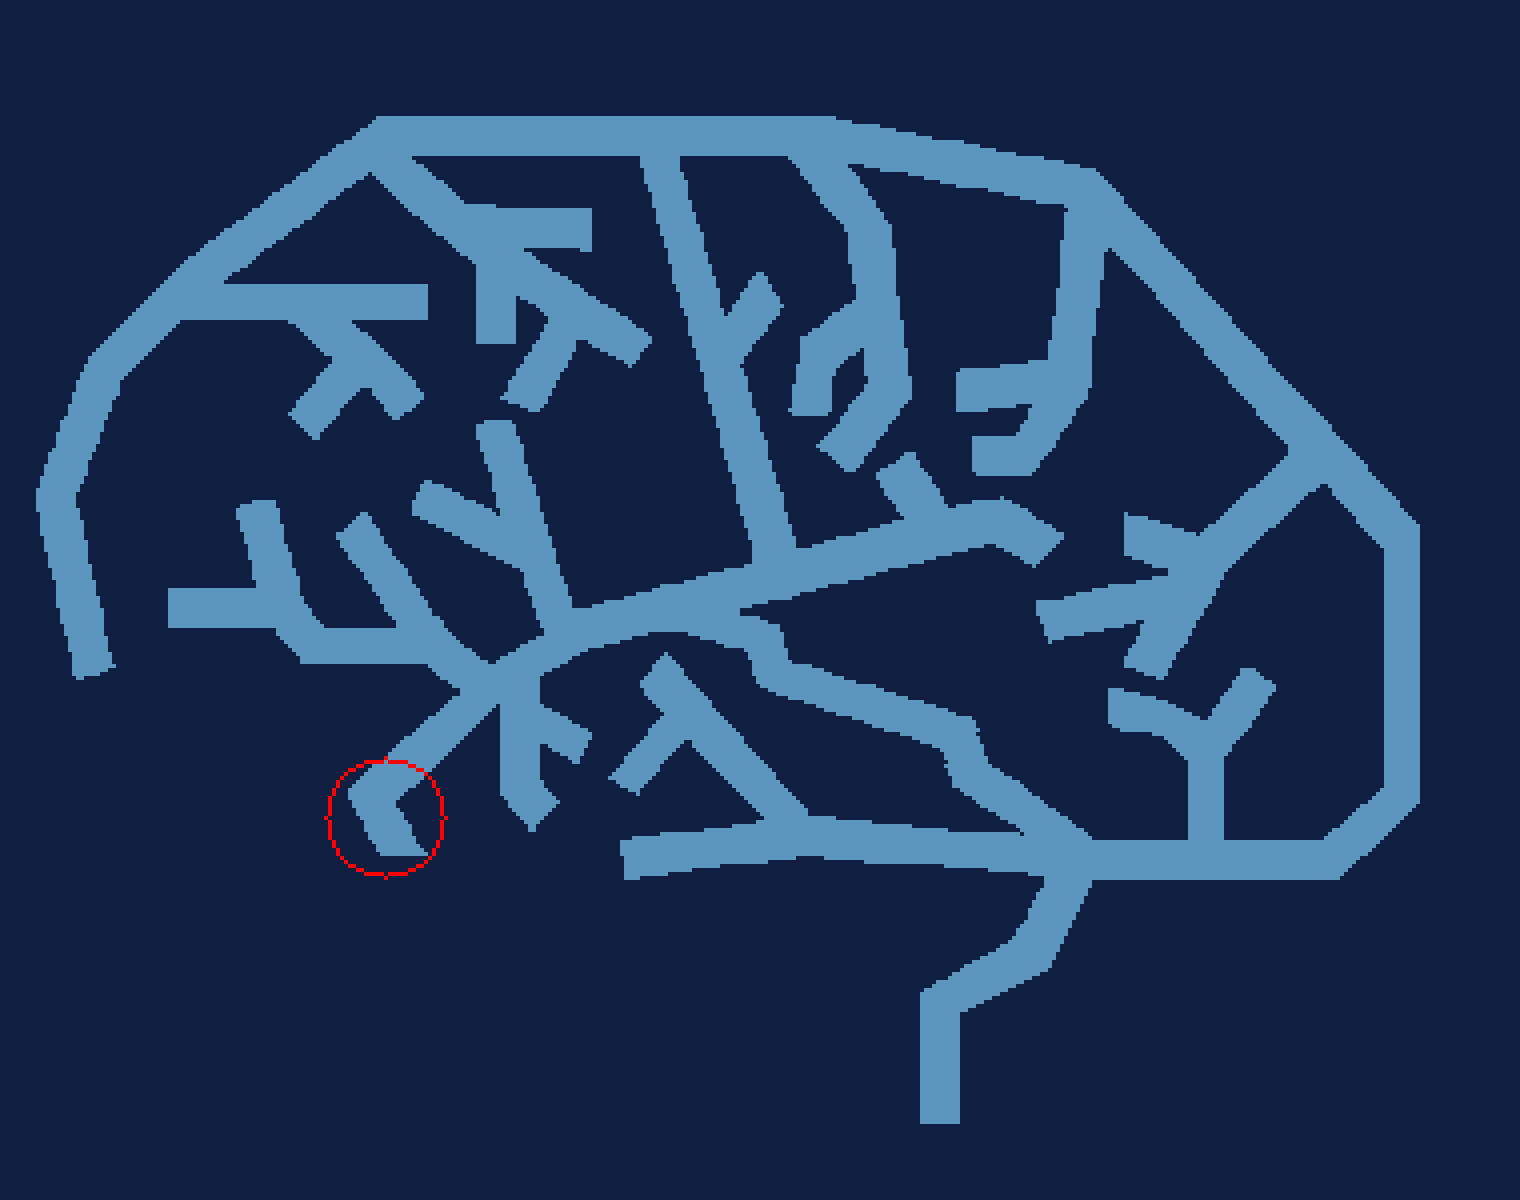
\includegraphics[clip, width=3.5cm]{figures/evaluation/procedure/brain_upscaled.png}} & Brain & $(380 \times 300)$ & $22593 \ (\approx 19.82\%)$ & 221.19 & 400 \\
            \addlinespace[0.05cm]
            \midrule
            
            \parbox[c]{3.5cm}{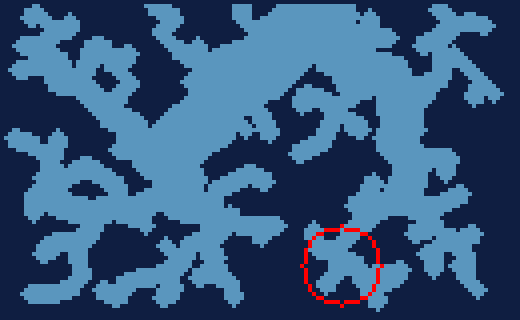
\includegraphics[clip, width=3.5cm]{figures/evaluation/procedure/vessel_upscaled.png}} & Vessel & $(130 \times 80)$ & $4949 \ (\approx 47.59\%)$ & 77.47 & 136 \\
            \addlinespace[0.05cm]
            \bottomrule
        \end{tabular}
    \end{center}
    \caption[Test Instances]{A list of our default test instances. Light blue pixels denote non-blocked pixels. The goal position is marked with a red circle. \textit{Dimension} describes the absolute size of the instance, while \textit{size} denotes the actual non-blocked area. We also included values for the average $d_{avg}$ and maximum $d_{max}$ distance between any point and the goal position.} \label{tab:TestInstances}
\end{table}

If not stated otherwise, we used 256 randomly generated particles for each episode during training. Episode lengths are capped at a maximum of 2000 steps independent of the environment. Dynamic episode lengths can also not exceed this hard cap.

\section{Reward Generation} \label{sec:EvalReward}
In this section we want to analyze how the reward generation influences training performance. In Section \ref{sec:RewardTestResults} we show our results and highlight key findings. We then continue to analyze some of the more important findings in Section \ref{sec:RewardAnalysis} and finish with our conclusion in Section \ref{sec:RewardConclusion}.

Since rewards are a key element to reinforcement learning, we expect that different rewards will heavily impact training performance. Our reward system provides a huge number of possible combinations of reward components and we therefore decide to use an iterative testing approach: We first test many combinations on the easy Corridor instance and then only evaluate the promising combinations on the Vessel instance. We finally select only the best performing combinations from the Vessel instance and test them on the Brain instance. Since observation normalization can have a huge impact on training performance and directly influences reward generation in the case of intrinsic reward, we also decided to add a second form of observation normalization in the form of $x \mapsto CLIP((x - \mu)/\sigma, [-10, 10])$ into this experiment. Note that the observation normalization of $x \mapsto x/255$ is always used if the second normalization option is not used.

Throughout this section we will provide a number of tables, which use abbreviations to save space. The abbreviations are explained in Table \ref{tab:RewardAbbreviations}.  

\begin{table} [ht]
    \begin{center}
        \small
        \begin{tabular}{ll}
            \toprule
            \multicolumn{1}{c}{Reward Component} & Abbreviation \\
            \midrule
            Continuous Reward & CR \\
            Discrete Reward & DR \\
            Observation Normalization & ON \\
            Reward Normalization & RN \\
            Time Penalty & TP \\
            Dynamic Episode Length & DEL \\
            Curiosity Reward & RND \\
            Gathering Reward & GR \\
            \bottomrule
        \end{tabular}
    \end{center}
    \caption[Abbreviations for Reward Components]{Common abbreviations for reward components} \label{tab:RewardAbbreviations}
\end{table}


\subsection{Test Results} \label{sec:RewardTestResults}

\paragraph{Corridor Environment.}
We begin with our easy instance Corridor. In our tests, we use the basic settings from Section \ref{sec:TestProcedure} and train for 3 million steps per trial. Table \ref{tab:Maze0318/Reward/Discrete} contains the results for discrete rewards and Table \ref{tab:Maze0318/Reward/Continuous} contains the results for continuous rewards.

Looking at the data, we can see, that many parameters do work very well and our dense discrete reward produces results which result in vastly shorter training times than in previous work \cite{huang2019}. Our initial experiments for discrete reward also show some interesting findings: 
\begin{itemize}
    \item \textbf{Normalization. } We found, that normalization has a huge impact on training performance. Normalizing the reward has a positive impact on its own (see Experiments 4/6), but additionally normalizing the observation by mean and standard deviation seems to be very important to improve performance in comparison to simple normalization (see Experiments 7/11 or 8/10).
    \item \textbf{Curiosity. } Using our relatively dense discrete reward, curiosity does not seem to have a positive effect for simple instances. Using DEL, a small amount of curiosity reward seems to have a positive impact (see Experiments 1/3), but also can have a negative impact if the weight is higher (see Experiments 1/2 or 13/14). Curiosity may have a greater impact when training with more complex instances though.
    \item \textbf{Dynamic Episode Length. } DEL does not seem to have any positive impact on the training performance. Experiment 9 shows that DEL is capable of creating time penalty like pressure, but the final result is worse than training with our normal time penalty. In combination with curiosity reward or a standard time penalty, performance seems to also worsen. (see Experiments 11/13; 12/14)
    \item \textbf{Gathering Reward. } Gathering reward does not seem to have any influence on the performance for small instances. Further testing will show, if this changes with larger or more challenging instances, where gathering of particles before bringing them to the goal might be more beneficial.
\end{itemize}


\begin{table}[htp]
    \begin{center}
        \begin{tabular}{rccccccrrr}
            \toprule
             & \multicolumn{6}{c}{Reward Component} & \multicolumn{2}{c}{Episode Length} & \\
            \cmidrule(lr){2-7}\cmidrule(lr){8-9}
            \multicolumn{1}{c}{Idx} & \multicolumn{1}{c}{ON} & \multicolumn{1}{c}{RN} & \multicolumn{1}{c}{TP} & \multicolumn{1}{c}{DEL} & \multicolumn{1}{c}{RND} & \multicolumn{1}{c}{GR} & \multicolumn{1}{c}{Best} & \multicolumn{1}{c}{Avg} & \multicolumn{1}{c}{Drop}\\
            \midrule
            1 &  &  &  & X &  &  & 256.78 & 295.04 & 1.25M \\
            2 &  &  &  & X & 0.50 &  & 499.97 & 499.99 & 750k \\
            3 &  &  &  & X & 0.25 &  & 110.94 & 117.82 & 750k \\
            4 &  &  & X &  &  &  & 135.03 & 145.34 & 629k \\
            5 &  &  & X &  & 0.25 &  & 324.29 & 422.48 & 456k \\
            6 &  &  & X & X &  &  & 477.62 & 491.48 & 3M \\
            7 &  & X & X &  &  &  & 83.78 & 84.66 & 461k \\
            8 &  & X & X &  &  & 1.00 & 93.31 & 94.30 & 406k \\
            9 & X & X &  & X &  &  & 65.72 & 67.17 & 400k \\
            10 & X & X & X &  &  & 1.00 & 59.31 & \textbf{65.68} & 190k \\
            11 & X & X & X &  &  &  & \textbf{57.38} & 66.81 & 182k \\
            12 & X & X & X &  & 0.50 &  & 84.52 & 207.78 & \textbf{181k} \\
            13 & X & X & X & X &  &  & 65.34 & 78.93 & 400k \\
            14 & X & X & X & X & 0.50 &  & 500.00 & 500.00 & 3M \\
            \bottomrule
        \end{tabular}
    \end{center}
    \caption[Evaluation of Discrete Reward Evaluation with the Corridor Environment]{Evaluation of discrete rewards with the corridor environment.} \label{tab:Maze0318/Reward/Discrete}
\end{table}


The evaluation results using continuous reward show similar outcomes to the experiments using discrete reward. The most important finding is, that the best continuous reward is able to produce superior results in every category compared to the best discrete reward. Especially the time of first notable improvement is about 30\% earlier. We included a plot showing the average episode length during training in Figure \ref{fig:ContinuousVsDiscrete}. This further supports our decision to create more dense rewards. 

\begin{table}[htp]
    \begin{center}
        \begin{tabular}{rccccccccrrr}
            \toprule
             & \multicolumn{8}{c}{Reward Component} & \multicolumn{2}{c}{Episode Length} & \\
            \cmidrule(lr){2-9}\cmidrule(lr){10-11}
            \multicolumn{1}{c}{Idx} & \multicolumn{1}{c}{ON} & \multicolumn{1}{c}{RN} & \multicolumn{1}{c}{TP} & \multicolumn{1}{c}{DEL} & \multicolumn{1}{c}{RND} & \multicolumn{1}{c}{GR} & \multicolumn{1}{c}{Int Norm} & \multicolumn{1}{c}{PO} & \multicolumn{1}{c}{Best} & \multicolumn{1}{c}{Avg} & \multicolumn{1}{c}{Drop}\\
            \midrule
            1 &  &  &  & X &  &  & X &  & 101.06 & 106.07 & 600k \\
            2 &  &  &  & X & 0.25 &  & X &  & 394.12 & 413.82 & 800k \\
            3 &  &  & X &  &  &  &  &  & 146.38 & 149.47 & 787k \\
            4 &  &  & X &  &  &  & X &  & 102.44 & 103.96 & 718k \\
            5 &  &  & X & X &  &  & X &  & 92.12 & 96.00 & 400k \\
            6 &  & X & X &  &  &  & X & X & 90.47 & 98.18 & 370k \\
            7 &  & X & X &  &  &  & X &  & 101.62 & 102.40 & 525k \\
            8 &  & X & X &  &  & 1.00 & X &  & 96.22 & 103.99 & 614k \\
            9 &  & X & X &  & 0.25 &  & X &  & 198.44 & 335.29 & 561k \\
            10 & X & X &  & X &  &  & X &  & 82.41 & 83.32 & 400k \\
            11 & X & X & X &  &  &  &  &  & \textbf{56.59} & \textbf{59.04} & \textbf{127k} \\
            12 & X & X & X &  &  &  & X & X & 58.72 & 65.46 & 152k \\
            13 & X & X & X &  &  &  & X &  & 61.81 & 71.28 & 147k \\
            14 & X & X & X &  &  & 1.00 &  &  & 60.53 & 62.46 & 149k \\
            15 & X & X & X &  &  & 1.00 & X &  & 59.09 & 68.69 & 151k \\
            16 & X & X & X &  & 0.25 &  & X & X & 69.41 & 246.38 & 158k \\
            17 & X & X & X & X &  &  & X & X & 79.19 & 79.39 & 400k \\
            \bottomrule
        \end{tabular}
    \end{center}
    \caption[Evaluation of Continuous Reward with the Corridor Environment]{Evaluation of continuous rewards with the corridor environment.} \label{tab:Maze0318/Reward/Continuous}
\end{table}


\begin{figure}[htp]
    
    \begin{center}
        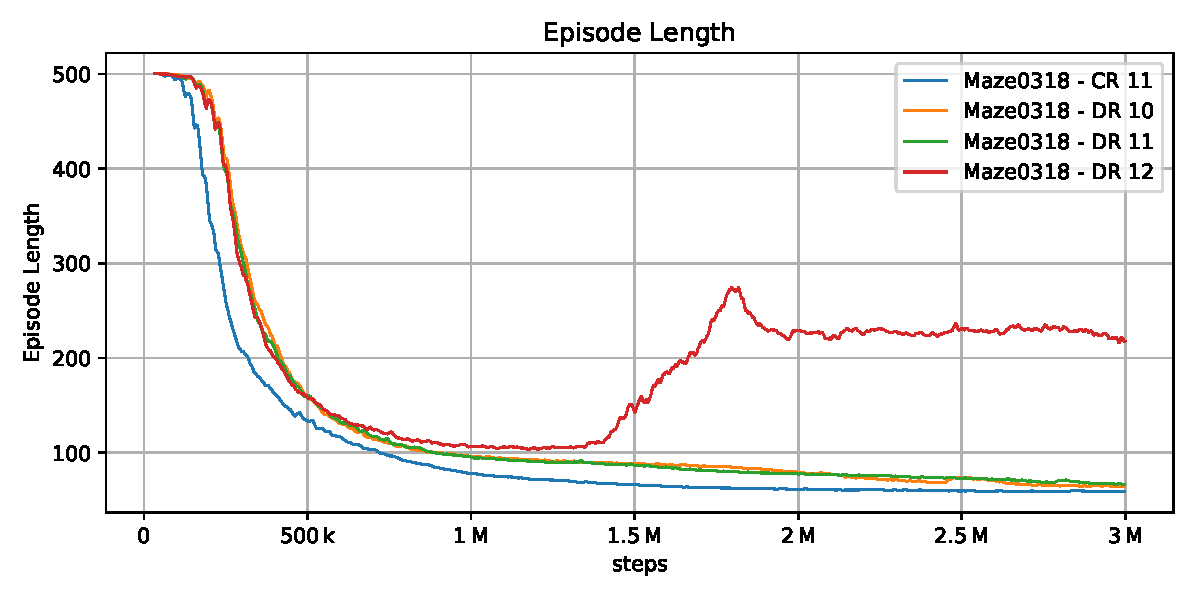
\includegraphics[clip, width=0.75\columnwidth]{figures/evaluation/rewards/continuous_vs_discrete.pdf}
    \end{center}
    
    %\vspace*{-6pt}
    \caption[Training Curves with Curiosity Reward]{Average episode length on the corridor environment during training. The legend refers to experiment numbers.}
    \label{fig:ContinuousVsDiscrete}
    %\vspace*{-12pt}
\end{figure}

\begin{figure}[htp]
    
    \begin{center}
        \begin{tabular}{c}
            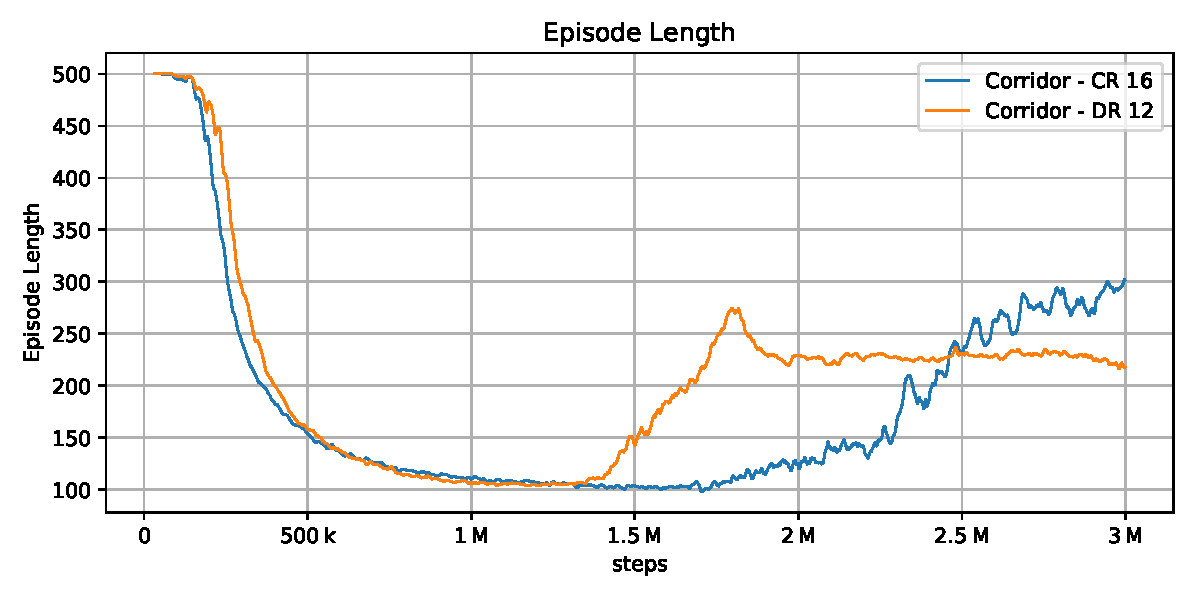
\includegraphics[clip, width=0.75\columnwidth]{figures/evaluation/rewards/curiosity_divergence_ep_len.pdf} \\
            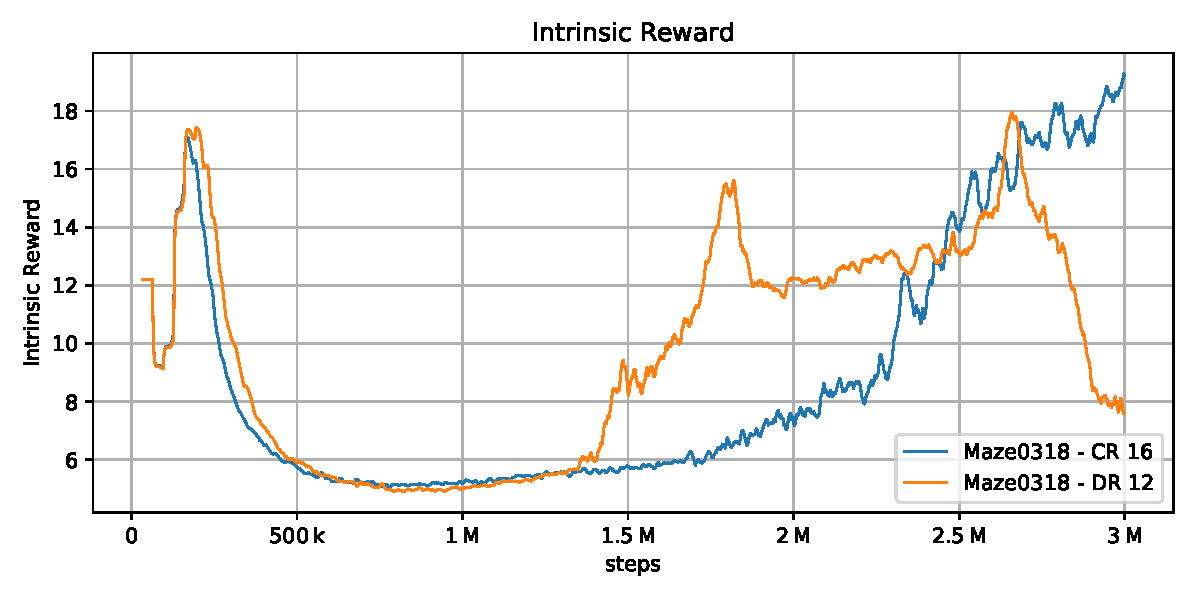
\includegraphics[clip, width=0.75\columnwidth]{figures/evaluation/rewards/curiosity_divergence_int_rew.pdf} \\
            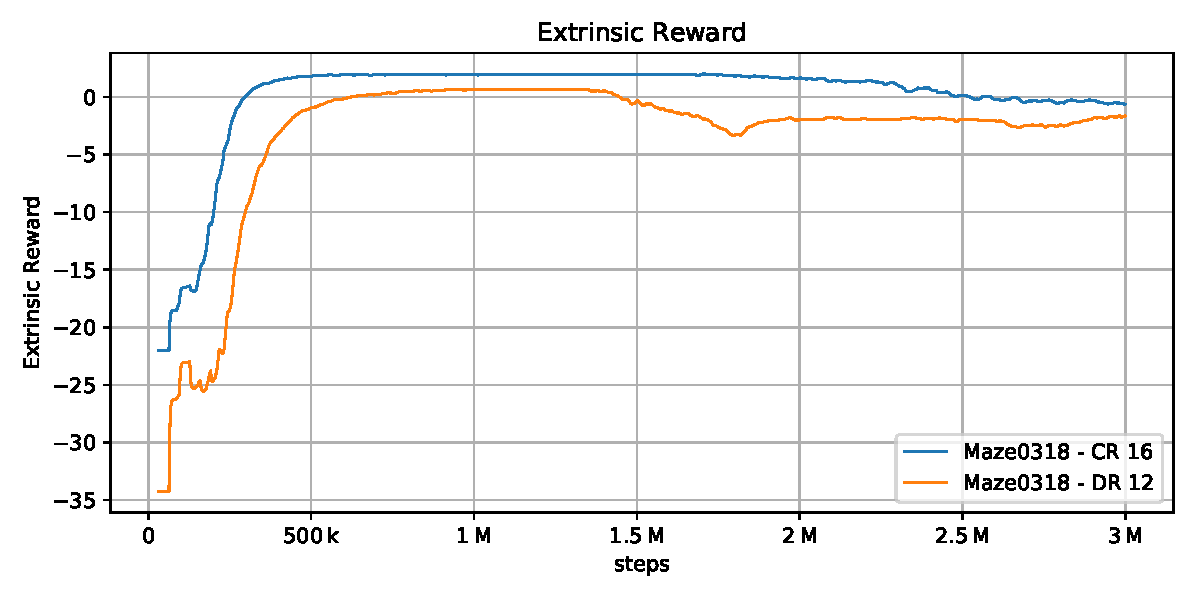
\includegraphics[clip, width=0.75\columnwidth]{figures/evaluation/rewards/curiosity_divergence_ext_rew.pdf}
        \end{tabular}

    \end{center}
    
    %\vspace*{-6pt}
    \caption[Problems with Curiosity Reward]{Learning curves for training with curiosity reward. We observed, that intrinsic rewards increase the chance for a performance collapse during training in terms of episode length. This can be seen, by comparing the intrinsic to the extrinsic reward and looking at the episode length at the same time: At around 1.5 million training steps, the intrinsic reward begins to increase, while the extrinsic reward remains at a constant level. At the same time, the average episode length begins to increase.}
    \label{fig:CuriosityDiverge}
    %\vspace*{-12pt}
\end{figure}


Similar to the results obtained when using discrete rewards, we can see, that observation normalization by mean and standard deviation massively improves performance for continuous rewards. Curiosity also does not seem to improve the results and often tends to diverge from the optimum at the end of training as shown in Figure \ref{fig:CuriosityDiverge}. Otherwise the corridor instance seems to be too easy to show differences between other reward parameters. Like before, gathering reward does not seem to have any positive or negative impact. The use of positive only rewards shows to improve performance without normalization (see Experiments 3/4), but only has a small impact with normalization (see Experiments 12/13). Interestingly internal normalization which balances the total cost reward against the maximum cost reward has shown to worsen the results on the corridor environment (see Experiments 11/13). 


\paragraph{Vessel Environment.} We repeat multiple experiments on the more complicated, but similarly large vessel instance. The results for discrete rewards are shown in Table \ref{tab:VesselMaze02/Reward/Discrete} and the results for continuous reward in Table \ref{tab:VesselMaze02/Reward/Continuous}. To compensate for the more complex environment, we double the training time for the agent and train for 6 millions steps per trial. 

Looking at the results for discrete rewards in Table \ref{tab:VesselMaze02/Reward/Discrete}, we can see, that normalization is crucial for success. While agents trained with non-normalized rewards are still able to find solutions, they need much more training time. For discrete rewards, the addition of a supporting reward signals seems to be important: The experiments including dynamic episode length (3), gathering reward (5) or curiosity reward (6) all produced better results, than stand-alone discrete reward (4). Especially the combination of discrete reward with curiosity was able to find a solution in a relatively short time. Note, that training with curiosity is significantly slower due to the extra computation for the training of the predictor network. 

\begin{table}[htp]
    \begin{center}
        \begin{tabular}{rccccccrrr}
            \toprule
             & \multicolumn{6}{c}{Reward Component} & \multicolumn{2}{c}{Episode Length} & \\
            \cmidrule(lr){2-7}\cmidrule(lr){8-9}
            \multicolumn{1}{c}{Idx} & \multicolumn{1}{c}{ON} & \multicolumn{1}{c}{RN} & \multicolumn{1}{c}{TP} & \multicolumn{1}{c}{DEL} & \multicolumn{1}{c}{RND} & \multicolumn{1}{c}{GR} & \multicolumn{1}{c}{Best} & \multicolumn{1}{c}{Avg} & \multicolumn{1}{c}{Drop}\\
            \midrule
            1 &  &  &  & X & 0.25 &  & 478.91 & 487.95 & 9.99M \\
            2 &  &  & X &  & 0.25 &  & 491.19 & 497.06 & 9.99M \\
            3 & X & X &  & X &  &  & \textbf{89.38} & 95.75 & 1.2M \\
            4 & X & X & X &  &  &  & 97.28 & 100.09 & 762k \\
            5 & X & X & X &  &  & 1.00 & 93.78 & \textbf{95.15} & 828k \\
            6 & X & X & X &  & 0.50 &  & 107.31 & 109.18 & \textbf{694k} \\
            7 & X & X & X & X &  &  & 89.62 & 96.38 & 1.2M \\
            \bottomrule
        \end{tabular}
    \end{center}
    \caption[Evaluation of Discrete Reward Evaluation with the Vessel Environment]{Evaluation of discrete rewards with the vessel environment.} \label{tab:VesselMaze02/Reward/Discrete}
\end{table}


The results for continuous rewards differ from the results for discrete rewards. By looking at Table \ref{tab:VesselMaze02/Reward/Continuous} we can see, that the addition of supporting rewards often produces worse results (see Experiments 7/11, 4/5, 8/10). An exception seems to be the combination of gathering reward with not internally normalized reward (see Experiments 6/9). Using only positive reward, does not seem to improve performance. The same is true for dynamic episode lengths.  


\begin{table}[htp]
    \begin{center}
        \begin{tabular}{rccccccccrrr}
            \toprule
             & \multicolumn{8}{c}{Reward Component} & \multicolumn{2}{c}{Episode Length} & \\
            \cmidrule(lr){2-9}\cmidrule(lr){10-11}
            \multicolumn{1}{c}{Idx} & \multicolumn{1}{c}{ON} & \multicolumn{1}{c}{RN} & \multicolumn{1}{c}{TP} & \multicolumn{1}{c}{DEL} & \multicolumn{1}{c}{RND} & \multicolumn{1}{c}{GR} & \multicolumn{1}{c}{Int Norm} & \multicolumn{1}{c}{PO} & \multicolumn{1}{c}{Best} & \multicolumn{1}{c}{Avg} & \multicolumn{1}{c}{Drop}\\
            \midrule
            1 &  &  & X &  & 0.25 &  & X &  & 451.00 & 476.26 & 7.92M \\
            2 &  & X & X &  &  &  &  &  & 423.09 & 433.16 & 7.81M \\
            3 &  & X & X &  &  &  & X & X & 373.28 & 405.12 & 8M \\
            4 &  & X & X &  &  &  & X &  & 416.28 & 458.89 & 7.91M \\
            5 &  & X & X &  &  & 1.00 & X &  & 418.75 & 470.94 & 7.05M \\
            6 & X & X & X &  &  &  &  &  & 93.97 & 98.73 & \textbf{501k} \\
            7 & X & X & X &  &  &  & X & X & 103.16 & 105.57 & 628k \\
            8 & X & X & X &  &  &  & X &  & 91.06 & \textbf{96.72} & 532k \\
            9 & X & X & X &  &  & 1.00 &  &  & \textbf{89.41} & 100.26 & 600k \\
            10 & X & X & X &  &  & 1.00 & X &  & 95.16 & 98.65 & 507k \\
            11 & X & X & X &  & 0.25 &  & X & X & 126.94 & 197.88 & 601k \\
            12 & X & X & X & X &  &  & X & X & 185.62 & 193.65 & 2.8M \\
            \bottomrule
        \end{tabular}
    \end{center}
    \caption[Evaluation of Continuous Reward with the Vessel Environment]{Evaluation of continuous rewards with the vessel environment.} \label{tab:VesselMaze02/Reward/Continuous}
\end{table}

\paragraph{Brain Environment.} We finally tested our the best performing reward configurations from the vessel environment on the brain environment. To compensate for the larger instance size and increased complexity, we again doubled training times, resulting in a total of 12 million training steps per trial. 

The results for discrete reward are listed in Table \ref{tab:Maze0122/Reward/Discrete}. Surprisingly, two of the three selected rewards did perform very poorly. Neither the configuration with dynamic episode length nor the one with curiosity reward did yield acceptable end results after 12 million training steps. The only discrete reward variation that can solve the brain environment successfully under the given time limit uses additional gathering reward. 


\begin{table}[htp]
    \begin{center}
        \begin{tabular}{rccccccrrr}
            \toprule
             & \multicolumn{6}{c}{Reward Component} & \multicolumn{2}{c}{Episode Length} & \\
            \cmidrule(lr){2-7}\cmidrule(lr){8-9}
            \multicolumn{1}{c}{Idx} & \multicolumn{1}{c}{ON} & \multicolumn{1}{c}{RN} & \multicolumn{1}{c}{TP} & \multicolumn{1}{c}{DEL} & \multicolumn{1}{c}{RND} & \multicolumn{1}{c}{GR} & \multicolumn{1}{c}{Best} & \multicolumn{1}{c}{Avg} & \multicolumn{1}{c}{Drop}\\
            \midrule
            1 & X & X &  & X &  &  & 500.00 & 500.00 & 12M \\
            2 & X & X & X &  &  & 1.00 & \textbf{311.44} & \textbf{319.23} & \textbf{7.15M} \\
            3 & X & X & X &  & 0.50 &  & 479.59 & 486.36 & 12M \\
            \bottomrule
        \end{tabular}
    \end{center}
    \caption[Evaluation of Discrete Reward with the Brain Environment]{Evaluation of discrete rewards with the brain environment.} \label{tab:Maze0122/Reward/Discrete}
\end{table}

In contrast to the discrete reward variations, all continuous reward configurations were able to solve the brain environment. As we can see from Table \ref{tab:Maze0122/Reward/Continuous}, the addition of gathering reward yields the best results, while internally normalized (balanced) continuous reward performs better than non-balanced reward.

\begin{table}[htp]
    \begin{center}
        \begin{tabular}{rccccccccrrr}
            \toprule
             & \multicolumn{8}{c}{Reward Component} & \multicolumn{2}{c}{Episode Length} & \\
            \cmidrule(lr){2-9}\cmidrule(lr){10-11}
            \multicolumn{1}{c}{Idx} & \multicolumn{1}{c}{ON} & \multicolumn{1}{c}{RN} & \multicolumn{1}{c}{TP} & \multicolumn{1}{c}{DEL} & \multicolumn{1}{c}{RND} & \multicolumn{1}{c}{GR} & \multicolumn{1}{c}{Int Norm} & \multicolumn{1}{c}{PO} & \multicolumn{1}{c}{Best} & \multicolumn{1}{c}{Avg} & \multicolumn{1}{c}{Drop}\\
            \midrule
            1 & X & X & X &  &  &  &  &  & 328.97 & 352.97 & 7.46M \\
            2 & X & X & X &  &  &  & X &  & \textbf{308.31} & 333.53 & 7.34M \\
            3 & X & X & X &  &  & 1.00 & X &  & 324.78 & \textbf{333.35} & \textbf{6.75M} \\
            \bottomrule
        \end{tabular}
    \end{center}
    \caption[Evaluation of Continuous Reward with the Brain Environment]{Evaluation of continuous rewards with the brain environment.} \label{tab:Maze0122/Reward/Continuous}
\end{table}


\subsection{Analysis} \label{sec:RewardAnalysis}
While it is easy to understand that dense rewards provide more information to the agent and thus produced superior results, other aspects are not as clear. In this section we want to analyze the learned behavior under different reward settings, to get a better understanding why certain configurations work better than others.

\paragraph{Curiosity.} Intrinsic reward has been the key to success for previous work, while our experiments showed a negative influence on training performance. To understand this, we analyzed how episodes are solved by agents trained with and without curiosity. In Figure \ref{fig:curiosity_ep_analysis} we show metrics taken at each step over the course of a single episode on the corridor environment. Both agents were trained using continuous reward, using the settings from Experiment 11 (without curiosity) and Experiment 16 (with curiosity) on the corridor environment. 

\begin{figure}[htp]
    \begin{center}
        \begin{tabular}{c}
            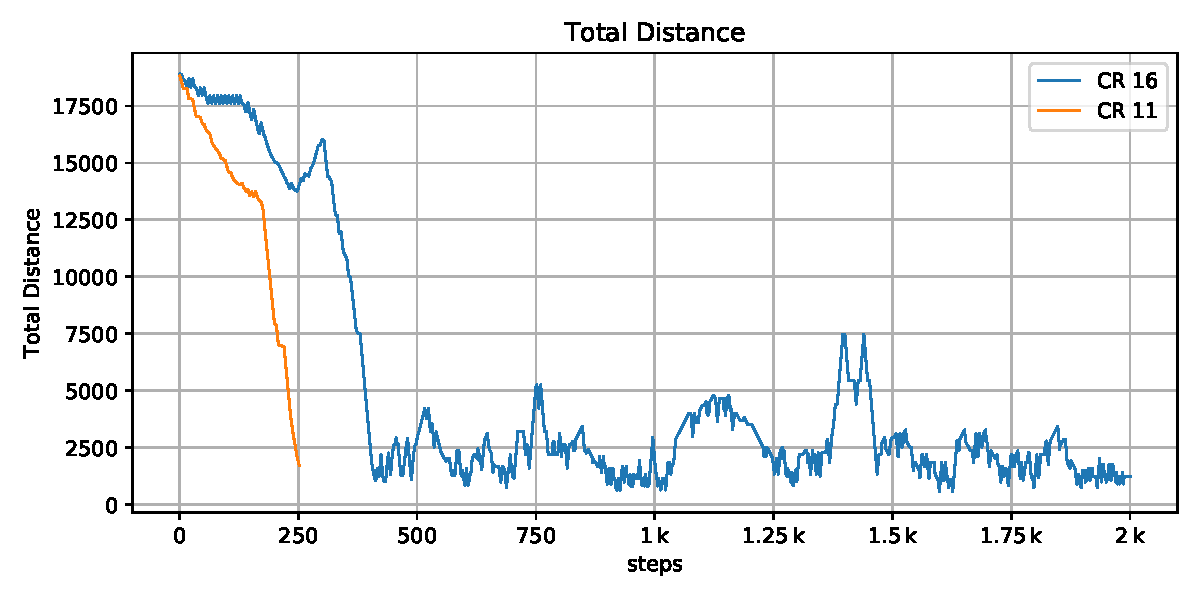
\includegraphics[clip, width=0.75\columnwidth]{figures/evaluation/rewards/episode_analysis/curiosity_total_distance.pdf} \\
            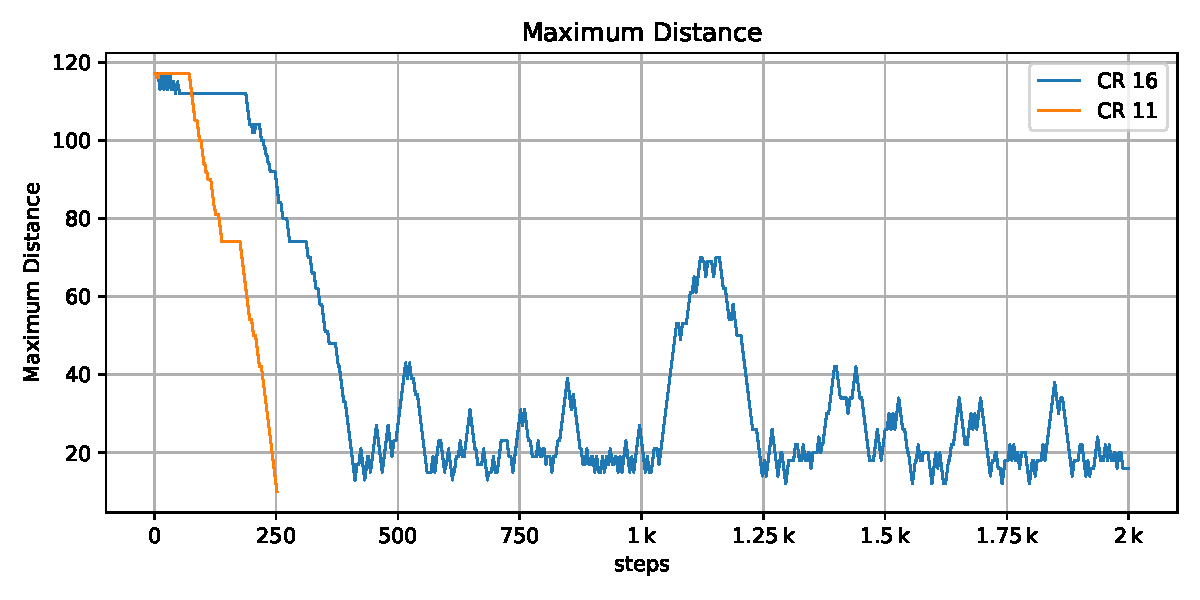
\includegraphics[clip, width=0.75\columnwidth]{figures/evaluation/rewards/episode_analysis/curiosity_max_distance.pdf} \\
            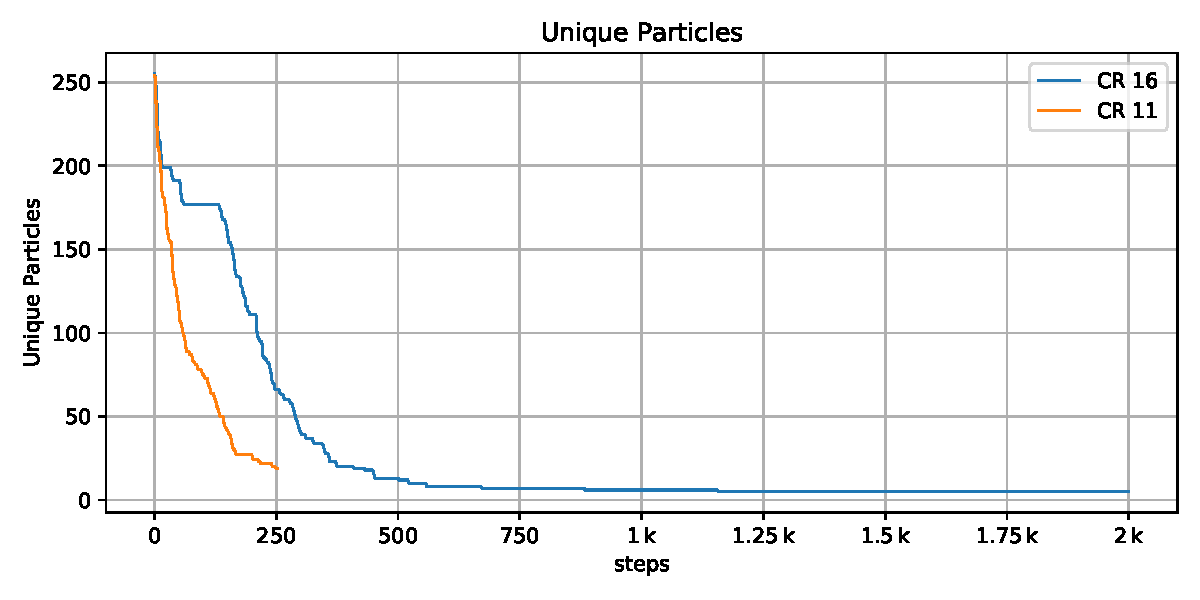
\includegraphics[clip, width=0.75\columnwidth]{figures/evaluation/rewards/episode_analysis/curiosity_unique_particles.pdf} \\
        \end{tabular}
    \end{center}
    \caption[Episode metrics on the Corridor Environment]{Metrics for a single example episode on the corridor instance. The steps are given without the MaxAndSkip wrapper and therefore in comparison 4 times larger. The blue line shows an agent trained with curiosity (see Experiment 16) and the orange line an agent trained without curiosity (see Experiment 11). The agent trained without curiosity is able to end the episode after about 250 steps, while the agent trained with curiosity does not end the episode during the 2000 steps time limit.} \label{fig:curiosity_ep_analysis}
\end{figure}


By looking at Figure \ref{fig:curiosity_ep_analysis} we can see, that both agents are able to reduce the total distance to the goal position very fast at the beginning of the episode. While the agent trained without curiosity finishes the episode after about 250 steps, the agent trained with curiosity decides to continue the episode by moving the particles back and forth close to the goal position. One could argue, that the agent might have to deal with a single particle that was left behind in the maze earlier, but this is not the case. We can see this by looking at the maximum distance any particle is away from the goal position. The particle which is the farthest away from the goal is closer than 20 pixels at around 470 steps and since the corridor environment only contains straight corridors, we can argue, that this particle cannot be stuck behind any obstacle. 

The question is why has the agent learned to not finish the episode when training with curiosity? We found, that there is a number of reasons why curiosity reward can be maximized by not finishing the episode. Let us begin with the easiest one: In Section \ref{sec:blRND} we showed, that an agent trained purely with curiosity learns to maximize episode lengths. Since it is able to explore more states during longer episodes, it can generate more intrinsic reward, if episodes are longer. The same happens in our particle environment where short episodes result in less intrinsic reward. Curiosity therefore works against our goal of achieving short episodes lengths. 

Another problem with curiosity comes from the nature of how the observations are generated in our environment: Since particles are directly shown in the observation and there are a lot of particles at the same time, the agent has control over a decent number of its own observation inputs. Since the agent is able to rapidly move the particles to appear at different positions, it is able to generate a massive amount of environment states and therefore observations similar to input noise. This situation is directly related to the \textit{noisy tv problem} described by Burda et al. \cite{burda2018large}. We can directly see this behavior in Figure \ref{fig:curiosity_ep_analysis}, where the agent has learned to increase the number of states, by gradually moving the particles to and away from the goal position, while slowly reducing the number of unique particles. Unfortunately this problem is not easy to fix. Implementing a large goal reward, may increase the number of episodes where the agent actually brings all particles to the goal, but the agent can still finish the episode at the last possible moment. Increasing the time penalty was found to help to some extend during our initial experiments. Previous experiments \cite{huang2019,becker2020} also used a larger time penalty and therefore may have not encountered this problem. Unfortunately we found that increasing the time penalty requires very careful fine-tuning for each environment to work correctly and therefore does not fix the underlying problem.

\paragraph{Observation Normalization. } Throughout our experiments, we observed large benefits from changing the observation normalization from normalization to the interval [0, 1] to normalization which also centers around zero by normalizing by $x \mapsto CLIP((x - \mu)/\sigma, [-10, 10])$. While normalization itself is a common technique in machine learning and has shown to improve training (e.g. \cite{jayalakshmi2011statistical}), for image-based tasks the normalization by mean and standard deviation is often used to compensate for brightness variation while still scaling the images to a smaller interval \cite{pal2016preprocessing}. 

In our case brightness variation is irrelevant, because our images are generated by our environment and do not change in brightness. So why does the agent still benefit from this normalization type? Because the area which is blocked by the maze never changes in value, when subtracting the mean from the input observation, the input becomes zero in all places where the maze blocks pixels. This makes it easier for the agent to ignore areas where no particles can be, because zero values in the input always mean zero activations in the network. Learning that an input value has no meaning is a harder task. The second reason is a benefit for the backpropagation algorithm, which works more stable, if it can work with zero centered input, since it allows the gradients to be both positive and negative.

\paragraph{Strategies.}
One interesting aspect for the future choice of rewards would be, if the learned strategies differ depending on the given reward. Looking at the change of total distance to the goal position in the brain environment (see Figure \ref{fig:Rewards/Ep_Analysis}), we can assume, that the learned strategies are pretty similar. Except for agents trained with the discrete reward in combination with DEL or curiosity, the change in distances is very similar.  

\begin{figure}[htp]
    \begin{center}
        \begin{tabular}{c}
            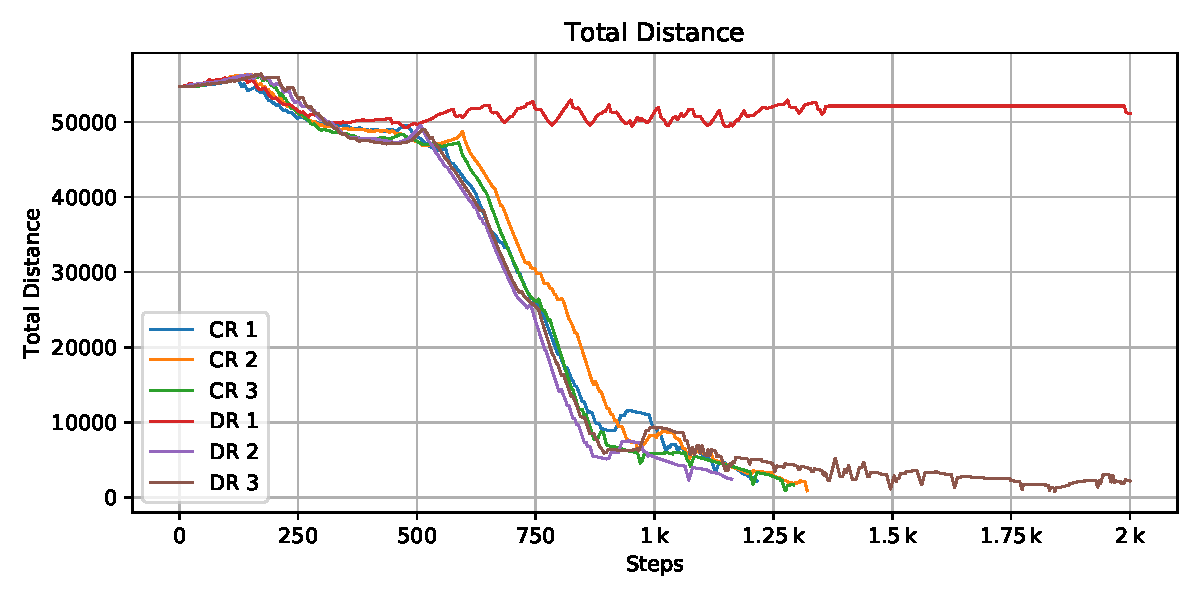
\includegraphics[clip, width=0.95\columnwidth]{figures/evaluation/rewards/episode_analysis/maze0122_total_dist.pdf} \\
            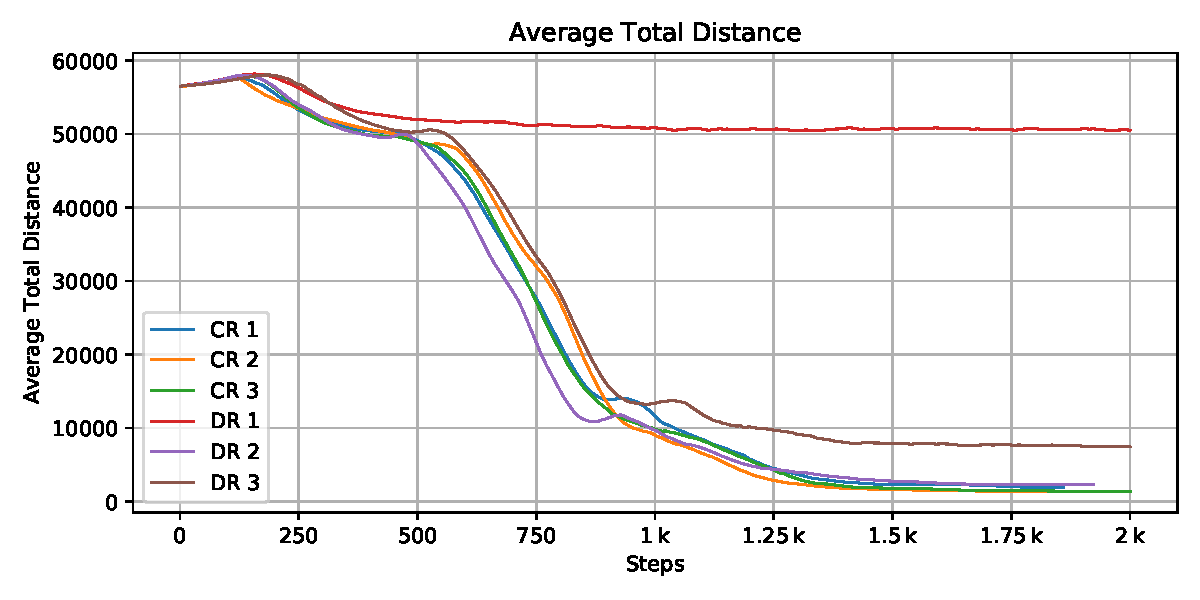
\includegraphics[clip, width=0.95\columnwidth]{figures/evaluation/rewards/episode_analysis/maze0122_total_dist_avg.pdf} \\
        \end{tabular}
    \end{center}
    \caption[Episode metrics on the Brain Environment]{Total sum of distances to the goal position over a single episode on the brain environment. On the top, we included a plot showing a single episode and on the bottom we included the average over 64 episodes.} \label{fig:Rewards/Ep_Analysis}
\end{figure}

To verify this result we monitor the similarity between actions for a given observation. We generate trajectories by replaying the different agents on the brain environment. We then replay the observations to all agents and count the differences in the choice of the best action (using stochastic policies). Note that an alternative measure would be to calculate an approximate Kullback-Leibler distance using the generated trajectories, but we found, that results are hard to interpret.

\begin{table}[htp]
    \begin{center}
        \begin{threeparttable}
            \begin{tabular}{l|rrrrrrr}
                \toprule
                vs & DR 2 & DR 2\tnote{1} & DR 3 & DR 1 & CR 2 & CR 3 & CR 1 \\
                \midrule
                DR 2 & 100.00 & 50.09 & 37.25 & 15.19 & 42.31 & 44.79 & 42.31 \\
                DR 2\tnote{1} & 50.09 & 100.00 & 45.41 & 10.89 & 39.33 & 43.84 & 45.83 \\
                DR 3 & 37.25 & 45.41 & 100.00 & 13.12 & 34.69 & 36.73 & 39.75 \\
                DR 1 & 15.19 & 10.89 & 13.12 & 100.00 & 15.68 & 18.43 & 15.10 \\
                CR 2 & 42.31 & 39.33 & 34.69 & 15.68 & 100.00 & 45.19 & 50.73 \\
                CR 3 & 44.79 & 43.84 & 36.73 & 18.43 & 45.19 & 100.00 & 48.54 \\
                CR 1 & 42.31 & 45.83 & 39.75 & 15.10 & 50.73 & 48.54 & 100.00 \\
                \bottomrule
            \end{tabular}
            \begin{tablenotes} \footnotesize
                \item[1] This agent uses the same reward as DR2, but from a different trial.
            \end{tablenotes}
        \end{threeparttable}
    \end{center}
    \caption[Agent Action Similarity for Different Rewards]{Similarity of actions between different agents given in percent of equal actions for the same observation on the brain environment. Similarity is measured by first generating observations by replaying the agents and then comparing the actions different agents would have chosen in the same situation.} \label{tab:Maze0122/Reward/Similarity}
\end{table}

We included the results in terms of percent of equal actions for the same observations in Table \ref{tab:Maze0122/Reward/Similarity}. A surprising result is, that two agents trained with the \textit{same} reward only produce the same action for about 50\% of the observations. The most reasonable explanation is that we have a set with very similar actions (e.g. NE, N, NW) and there are many situations where either of these actions can be used. Different neural networks then evolved into using only one of them for a specific input and therefore produce very dissimilar results for the same observation, even when trained with the same reward. Keeping this baseline in mind, we can see, that agents trained with different rewards also differ in their percentage of equal actions. Most notably the both worst performing agents trained with discrete reward (DR 1 and DR 3). For all other agents, the differences are significantly smaller. We can observe, that the agents using internally normalized (CR 2) and not internally normalized reward (CR 1) essentially learned the same strategy since they agree on even more observations than the two agents trained with DR 2. Adding gathering reward seems to lead to a slightly different strategy with between 2 and 5 percent of different action choices. 

Overall the choices of all agents which also yield good performance are relatively close. We can therefore assume, that the learned strategies only differ slightly and the agents all evolved into learning an similar optimized strategy independent of the used reward. 

\subsection{Conclusion} \label{sec:RewardConclusion}
When deciding for a reward for our further experiments, we have to keep in mind, that every extra computation will be executed for each individual training step. The more reward components we use, the longer training will take. When comparing the results on the brain environment for continuous reward, we saw that the addition of gathering reward just slightly improves the average end result. If we look at the wall-clock time, a single trial on the brain environment using the gathering reward took an average of 4:54h to complete, while a trial using only the continuous reward took 4:27h on average. This means that with gathering reward, we saw an increase of about 10\% more time. While additional components might provide benefits for special environments (see Section \ref{sec:EvalRandomness}) they do not provide significant improvements for our general case. Depending on the environment size, multiple rewards can be used to achieve good performance, but only a few scale well into larger instances. We therefore will use continuous internally normalized reward for all further experiments.

\section{RL Algorithms} \label{sec:EvalRLAlgorithms}
In this section we want to evaluate how different RL algorithms perform when solving maze environments. We presented a number of algorithms in Chapter \ref{chp: RLOverview} and want to test some of the most recent approaches including DQN (see Section \ref{ssec:DeepQLearning}), PPO (see Section \ref{ssec:PPO}), ACER and ACKTR (see Section \ref{ssec:AlternativeCombinedMethods}). Since the performance of most RL algorithms is very sensitive to the chosen hyperparameters, we optimized the parameters for each individual algorithm on the Vessel instance. This optimization included a wide range of parameters which were preselected using our automated hyperparametersearch system. We then used manual fine-tuning to get an optimal configuration for each algorithm. 

The parameters we selected for DQN, ACER and ACKTR can be found in Table \ref{tab:RLHyperparameters}. For PPO, we found that the parameters we choose during our initial experiments were already suited to yield good results and we will therefore use the parameters given in Table \ref{tab:PPOHyperparemeters}. PPO was also found to work with a wide range of parameters, e.g. increasing the number of optimization epochs could yield faster initial results, but is very time-consuming. We also tried to increase the number of parallel environments, but found that this does not further improve performance.  Decreasing the number of steps also has a positive initial effect, but worsens the final result.

\begin{table}[htp]
    \begin{center}
        \begin{threeparttable}
            \begin{tabular}{c}
                \begin{tabular}{|m{6cm}|R{2.5cm}|}
                    \hline
                    \multicolumn{1}{|c|}{Hyperparameter} & \multicolumn{1}{c|}{Value} \\
                    \hline
                    Rollout Length & 16 \\
                    Buffer Size & 5000 \\
                    Entropy Coefficient & 0.0001 \\
                    $\gamma$ & 0.98 \\
                    Learning Rate & 0.0007 \\
                    Learning Rate Schedule & Linear \\
                    Optimization Algorithm & RMSProp \cite{tieleman2012lecture} \\
                    Q Coefficient & 0.6 \\
                    Replay Ratio & 4 \\
                    Replay Start & 1000 \\
                    \hline
                \end{tabular} \\
                \addlinespace[0.15cm]
                {\small (a) Hyperparameters for ACER} \\
                \addlinespace[0.5cm]
                \begin{tabular}{|m{6cm}|R{2.5cm}|}
                    \hline
                    \multicolumn{1}{|c|}{Hyperparameter} & \multicolumn{1}{c|}{Value} \\
                    \hline
                    Rollout Length & 32 \\
                    Entropy Coefficient & 0.01 \\
                    $\gamma$ & 0.99 \\
                    $\lambda$ & 0.99 \\
                    Learning Rate & 0.2 \\
                    Value Function Coefficient & 0.25 \\
                    \hline
                \end{tabular} \\
                \addlinespace[0.15cm]
                {\small (b) Hyperparameters for ACKTR} \\
                \addlinespace[0.5cm]
                \begin{tabular}{|m{6cm}|R{2.5cm}|}
                    \hline
                    \multicolumn{1}{|c|}{Hyperparameter} & \multicolumn{1}{c|}{Value} \\
                    \hline
                    Learning Rate & 0.0005 \\
                    Learning Starts & 1000 \\
                    Target Network Update Frequency & 1000 \\
                    Train Frequency & 4 \\
                    Exploration Fraction & 0.5 \\
                    Exploration Final Epsilon & 0.05 \\
                    Buffer Size & 150000 \\
                    Prioritized Replay $\alpha$ & 0.6 \\
                    Prioritized Replay $\beta$ & 0.4 \\
                    \hline
                \end{tabular} \\
                \addlinespace[0.15cm]
                {\small (c) Hyperparameters for DQN\tnote{1} \ \tnote{2}} \\
    
            \end{tabular}
            \begin{tablenotes} \footnotesize
                \item[1] The DQN implementation of stable-baselines uses Double DQN and Dueling DQN.
                \item[2] We removed frame stacking and observation normalization for DQN as we found that it worsens results.
            \end{tablenotes}
        \end{threeparttable}
        
    \end{center}
    \caption[Hyperparameters]{Hyperparameters used for different RL Algorithms.} \label{tab:RLHyperparameters}
\end{table}

\subsection{Results}

Similar to previous experiments we tested the RL algorithms on our three test instances. The results for the Corridor instance can be found in Table \ref{tab:AlgorithmEval/Maze0318}, the results for the Vessel instance in Table \ref{tab:AlgorithmEval/VesselMaze02} and the results for the Brain instance in Table \ref{tab:AlgorithmEval/Maze0122}. Looking at the data, we can see, that three of our four algorithms performed well during the tests, namely ACER, ACKTR and PPO. DQN failed to deliver results even for the smallest instance and also took very long for each trial.

\begin{table}[htp]
    \begin{center}
        \begin{tabular}{rcrrrrr}
            \toprule
            \multicolumn{1}{c}{Idx} & \multicolumn{1}{c}{Algorithm} & \multicolumn{1}{c}{Best} & \multicolumn{1}{c}{Avg} & \multicolumn{1}{c}{Drop} & \multicolumn{1}{c}{Time}\\
            \midrule
            1 & PPO & 61.81 & 71.28 & 147k & 0:40:36h \\
            2 & DQN & 500.00 & 500.00 & 381k & 3:08:00h \\
            3 & ACKTR & 63.38 & 70.73 & 424k & \textbf{0:32:49h} \\
            4 & ACER & \textbf{55.84} & \textbf{68.83} & \textbf{100k} & 0:41:40h \\
            \bottomrule
        \end{tabular}
    \end{center}
    \caption[Evaluation of RL Algorithms on the Corridor Instance]{Evaluation results for different RL algorithms on the Corridor instance. We can see that ACER produced the best end results while also providing a fast initial improvement. In terms of wall-clock time, ACKTR provided the fastest results. DQN failed to solve the instance during our model evaluation episodes, but was able to solve some episodes during training (therefore the drop is below 3M).} \label{tab:AlgorithmEval/Maze0318}
\end{table}

\begin{table}[htp]
    \begin{center}
        \begin{tabular}{rcrrrrr}
            \toprule
            \multicolumn{1}{c}{Idx} & \multicolumn{1}{c}{Algorithm} & \multicolumn{1}{c}{Best} & \multicolumn{1}{c}{Avg} & \multicolumn{1}{c}{Drop} & \multicolumn{1}{c}{Time}\\
            \midrule
            1 & PPO & \textbf{91.06} & \textbf{96.72} & 532k & 1:10:00h \\
            2 & DQN & 500.00 & 500.00 & 6M & 5:40:24h \\
            3 & ACKTR & 103.88 & 109.20 & 759k & \textbf{0:51:54h} \\
            4 & ACER & 111.72 & 117.50 & \textbf{182k} & 1:12:57h \\
            \bottomrule
        \end{tabular}
    \end{center}
    \caption[Evaluation of RL Algorithms on the Vessel Instance]{Evaluation results for different RL algorithms on the Vessel instance. PPO is able to train the best performing agent, while ACKTR produces the fastest training times and ACER provides the fastest initial improvement. DQN again fails to deliver usable results.} \label{tab:AlgorithmEval/VesselMaze02}
\end{table}

\begin{table}[htp]
    \begin{center}
        \begin{tabular}{rcrrrrr}
            \toprule
            \multicolumn{1}{c}{Idx} & \multicolumn{1}{c}{Algorithm} & \multicolumn{1}{c}{Best} & \multicolumn{1}{c}{Avg} & \multicolumn{1}{c}{Drop} &  \multicolumn{1}{c}{Time}\\
            \midrule
            1 & PPO & \textbf{308.31} & \textbf{333.53} & \textbf{7.34M} & \textbf{4:28:39h} \\
            2 & ACKTR & 341.78 & 367.42 & 9.12M & 4:32:15h \\
            3 & ACER & 500.00 & 500.00 & 12M & 4:51:40h \\
            \bottomrule
        \end{tabular}
    \end{center}
    \caption{Evaluation results for different RL algorithms on the Brain instance. PPO delivers the best results in all categories (bold), delivering the best results in the shortest time. ACER fails to solve larger instances and may need more time or specific fine-tuning.} \label{tab:AlgorithmEval/Maze0122}
\end{table}

When comparing the other algorithms, we an see, that they all show certain strengths and weaknesses. ACER is able to provide very good results on the small Corridor instance, while also being the fastest in terms of initial improvement on both the Corridor and the Vessel instance. However ACER fails to solve the larger and more complex Brain instance during 12 million steps of training. ACKTR only provides average end results, while the algorithm is surprisingly fast in terms of wall-clock time. PPO shows to have the best overall performance, delivering the best results on the Vessel and Brain instance while still maintaining a reasonably good performance in terms of speed.   

\subsection{Analysis}
A surprising result for our experiments is that DQN was not able to solve even the easiest instance Corridor. Looking at the average episode length during training (see Figure \ref{fig:Algorithm/Ep_Length}) we see, that DQN was able to solve the environment at multiple points during training, but suffered from multiple training collapses. Interestingly the network trained with DQN was not able to solve the environment at test time during training. This means, that the DQN agent always relied on certain randomness coming from the epsilon-greedy strategy to randomly solve the maze. Because there exist a lot more DQN extensions which especially improve exploration, we suggest that a more powerful implementation of DQN might yield better results in the future.

\begin{figure}[htp]
    \begin{center}
        \begin{tabular}{c}
            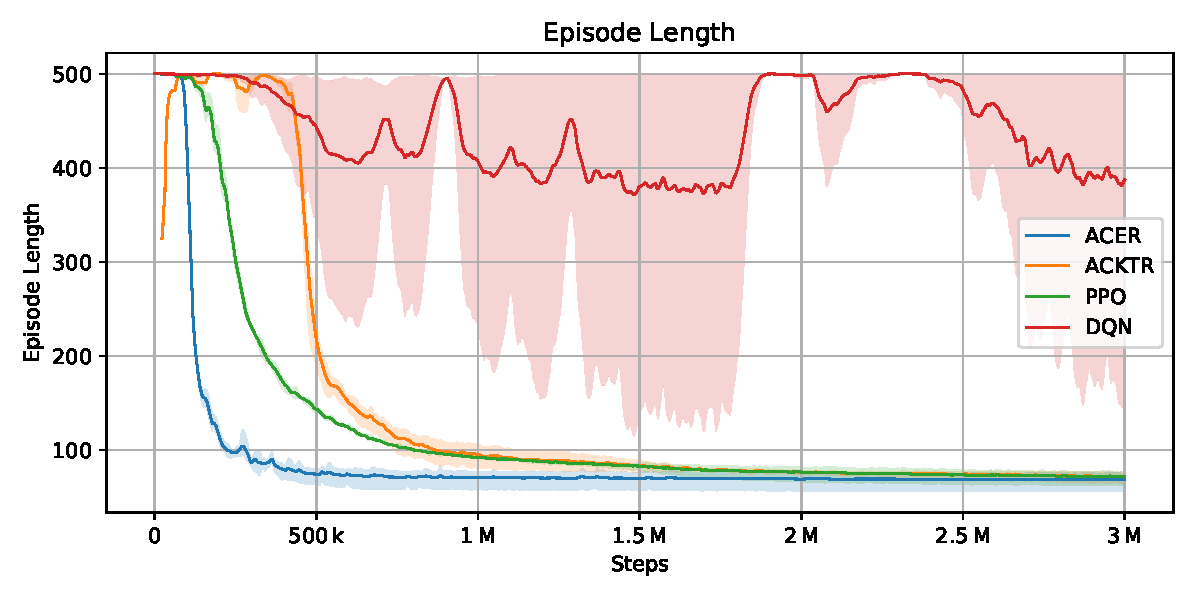
\includegraphics[clip, width=0.75\columnwidth]{figures/evaluation/algorithms/maze0318_episode_length.pdf} \\
            {\small (a) Episode length of different RL algorithms on the Corridor instance} \\
            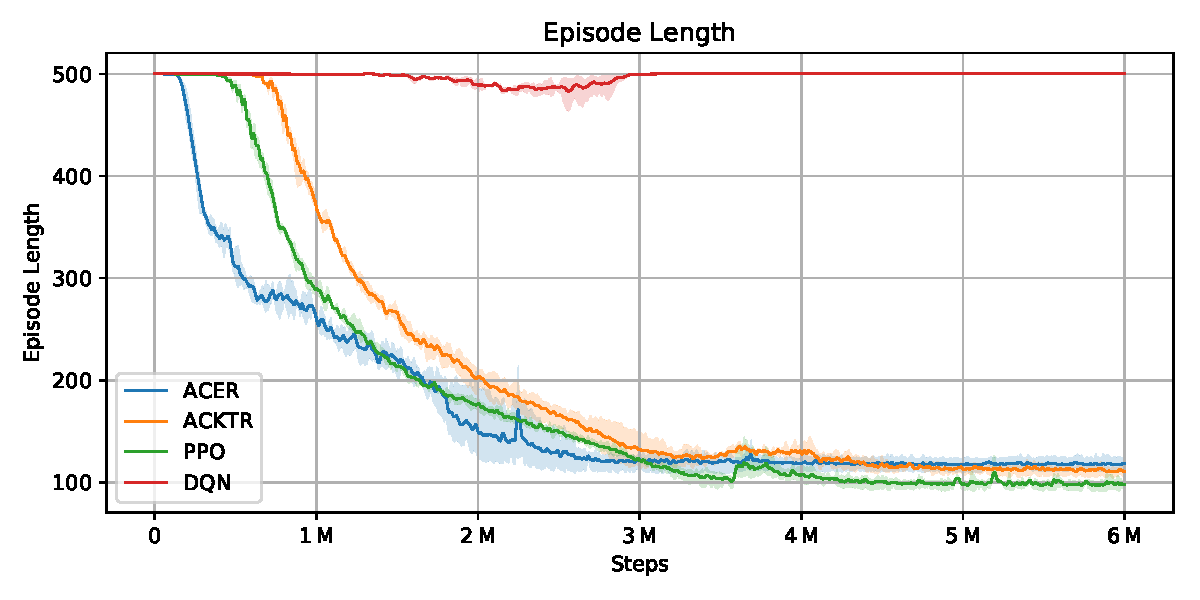
\includegraphics[clip, width=0.75\columnwidth]{figures/evaluation/algorithms/vesselmaze02_episode_length.pdf} \\
            {\small (b) Episode length of different RL algorithms on the Vessel instance} \\
            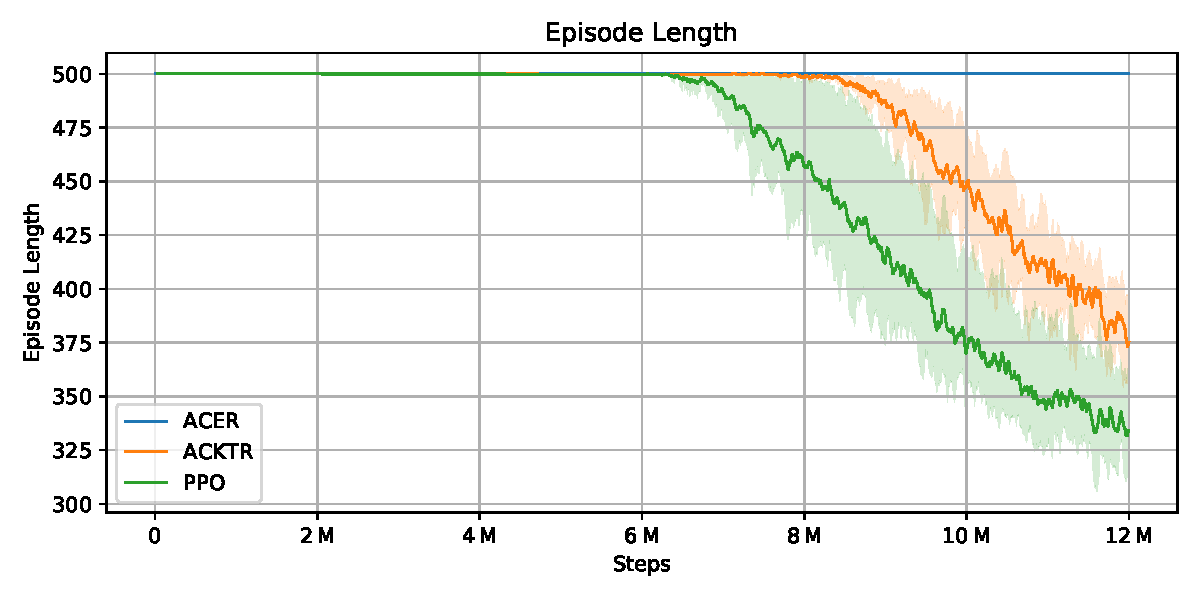
\includegraphics[clip, width=0.75\columnwidth]{figures/evaluation/algorithms/maze0122_episode_length.pdf} \\
            {\small (c) Episode length of different RL algorithms on the Brain instance} \\
        \end{tabular}
    \end{center}
    \caption[Episode Length During Training on the Test Environment]{Average episode length during training on our three test environments. We can see, that DQN is able to solve the easier instances at some point, but later suffers from training collapses. ACER is able to make very fast progress on Corridor and Vessel, but fails to solve Brain. PPO and ACKTR both solve all instances, with PPO delivering superior results in a smaller number of steps.} \label{fig:Algorithm/Ep_Length}
\end{figure}

\paragraph{Training Progress}
Figure \ref{fig:Algorithm/Ep_Length} shows the average episode length during training with different RL algorithms for our three test instances. Looking at Figure \ref{fig:Algorithm/Ep_Length} (a), we can see that DQN was able to compute solutions at various points during training, but suffered from performance collapses multiple times and was therefore unable to converge to a good final solution. All other algorithms were able to compute good solutions during the first one million training steps and then slowly optimized their results. 

\begin{figure} [htp]
    \begin{center}
        \begin{tabular}{c}
            \begin{tabular}{ccc}
                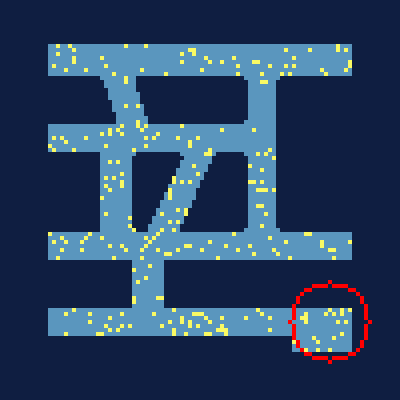
\includegraphics[width=0.26\columnwidth]{figures/evaluation/algorithms/training_example/acktr/0_k.png} & 
                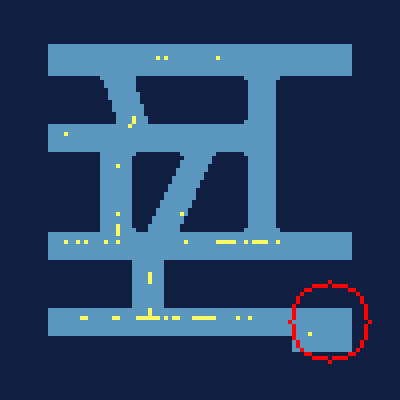
\includegraphics[width=0.26\columnwidth]{figures/evaluation/algorithms/training_example/acktr/6_k.png} & 
                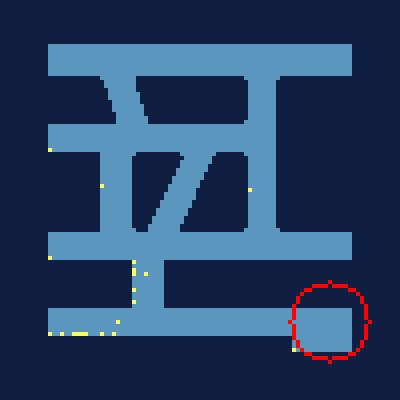
\includegraphics[width=0.26\columnwidth]{figures/evaluation/algorithms/training_example/acktr/12_k.png} \\
                \addlinespace[0.2cm]
                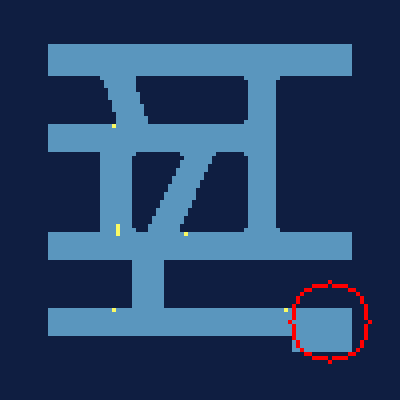
\includegraphics[width=0.26\columnwidth]{figures/evaluation/algorithms/training_example/acktr/18_k.png} &
                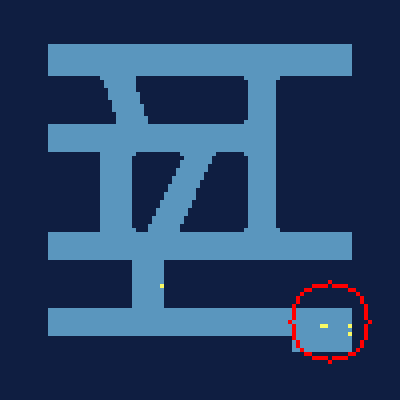
\includegraphics[width=0.26\columnwidth]{figures/evaluation/algorithms/training_example/acktr/25_k.png} & 
                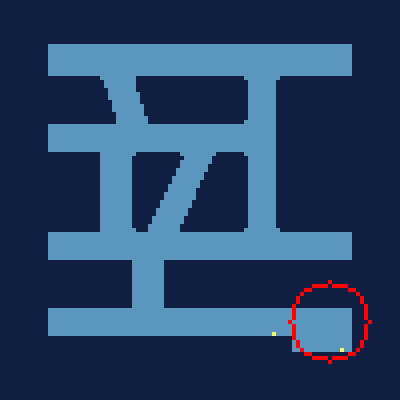
\includegraphics[width=0.26\columnwidth]{figures/evaluation/algorithms/training_example/acktr/29_k.png} \\
            \end{tabular} \\
            \addlinespace[0.1cm]
            {\small (a) Images from the first episode of training.} \\
            \addlinespace[0.5cm]
            \begin{tabular}{ccc}
                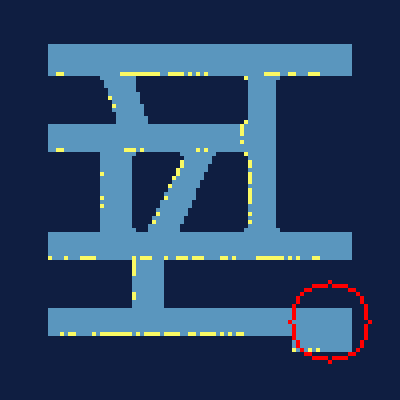
\includegraphics[width=0.26\columnwidth]{figures/evaluation/algorithms/training_example/acktr/30_k.png} & 
                
\includegraphics[width=0.26\columnwidth]{figures/evaluation/algorithms/training_example/acktr/37_k.png} & 
                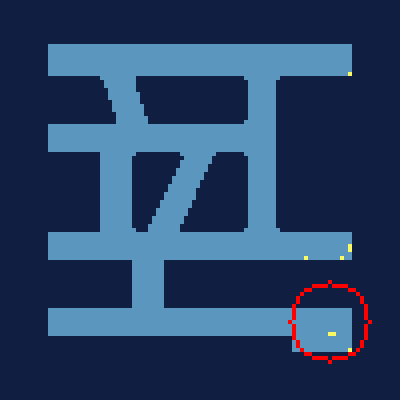
\includegraphics[width=0.26\columnwidth]{figures/evaluation/algorithms/training_example/acktr/44_k.png} \\
                \addlinespace[0.2cm]
                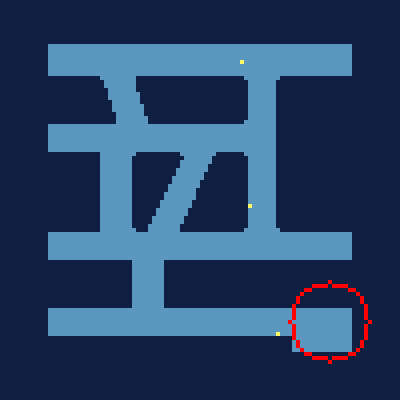
\includegraphics[width=0.26\columnwidth]{figures/evaluation/algorithms/training_example/acktr/51_k.png} &
                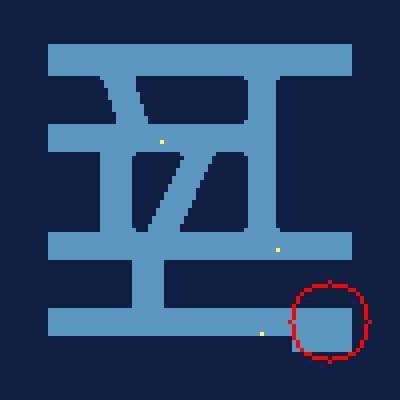
\includegraphics[width=0.26\columnwidth]{figures/evaluation/algorithms/training_example/acktr/58_k.png} & 
                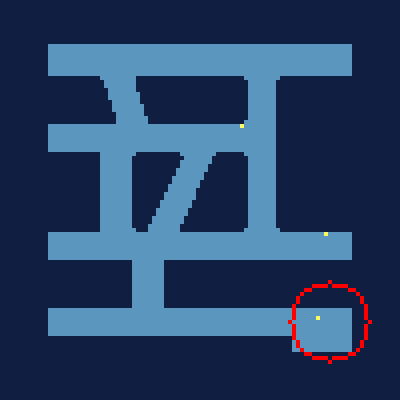
\includegraphics[width=0.26\columnwidth]{figures/evaluation/algorithms/training_example/acktr/65_k.png} \\
            \end{tabular} \\
            \addlinespace[0.1cm]
            {\small (b) Images from the second episode of training.} \\
        \end{tabular}
    \end{center}
    \caption[Images During Training Episodes with ACKTR]{Images from the first two episodes of training using ACKTR (from one of the 64 parallel environments). ACKTR improves the strategy of the agent each 32 steps, changing it about 15 times during a single episode. The first episode (a) is largely dominated by the random actions of the new neural network, but still delivers the particles to the goal, because ACKTR quickly favors actions moving particles down and \textit{later} actions moving particles right. The second episode (b) includes the knowledge from the first episode, but moving particles to the right too early leads to particles getting stuck in the corridor above the bottom corridor.} \label{fig:AcktrTrainingEpisodes}
\end{figure}


Looking at the training curve for ACKTR we can see a surprising unexpected result at the beginning of the training process: The average episode length is below the threshold of 500 steps at the beginning of training and then rises back to the maximum, before it drops again at around 500 thousand steps into training. To explain this anomaly, we included a series of images in Figure \ref{fig:AcktrTrainingEpisodes}, showing frames from the initial episodes generated during training. Figure \ref{fig:AcktrTrainingEpisodes} (a) shows images from the very first episode during training. The ACKTR agent trains its network every 32 steps, improving the network several times over the course of one episode. Because the network is only trained for a short time and stochastic actions are used during training, the agent is able to solve some of the 64 parallel environments, by quickly learning to choose actions that move particles downwards and later more actions which move particles to the right. After finishing the episode the agent learned, that going down and right somehow maximizes its reward and repeats this process. Unfortunately, going to the right too early brings particles into a place, where they are stuck and can only be moved to the goal, by going left (see Figure \ref{fig:AcktrTrainingEpisodes} (b)). Because this is the opposite of what the agent learned so far and it does not directly generate positive reward, due to other particles being moved away from the goal, the agent then struggles to learn this new behavior for the next few episodes.

Figure \ref{fig:Algorithm/Ep_Length} (b) and (c) show the average episode length during training for the Vessel and Brain environment. We can see that ACER optimizes faster for smaller instances, but fails to perform on the larger Brain instance. The curves for PPO and ACKTR seem to be pretty similar, with PPO always delivering results in less steps than ACKTR. This is most probably because the ACKTR implementation does not support the usage of multiple optimization epochs and is therefore less sample efficient than the PPO implementation. 

\begin{figure} [htp]
    \begin{center}
        \includegraphics[width=0.45\columnwidth]{figures/evaluation/algorithms/training_example/vessel/vessel_problems.png}
    \end{center}
    \caption[Training Challenges in the Vessel Environment]{Training challenges in the Vessel environment. After 100k training steps, all algorithms tend to already deliver a decent number of particles to the goal position. The rest of the training then is focused on learning movements to also bring particles to the goal which get stuck in the process and often require movements which bring particles away from the goal position. We highlighted spots where particles often get stuck in \textit{orange}.} \label{fig:Algorithm/Problems/Vessel}
\end{figure}


\begin{figure} [htp]
    \begin{center}
        \begin{tabular}{cc}
            \includegraphics[width=0.45\columnwidth]{figures/evaluation/algorithms/training_example/brain/brain_first_progress.png} & 
            \includegraphics[width=0.45\columnwidth]{figures/evaluation/algorithms/training_example/brain/brain_problem_1.png} \\
        \end{tabular}
    \end{center}
    \caption[Training Challenges in the Brain environment]{Training challenges in the Brain environment. Algorithms learn to gather particles at the position marked in green after 100k training steps (left). During this gathering process a number of particles gets stuck at the positions marked in orange. The right image shows the agents behavior after 3 million training steps. The agent has improved its gathering strategy and tries to bring the particles closer to the goal by moving them along the green path. In the process, particles get stuck at positions marked in orange.} \label{fig:Algorithm/Problems/Brain}
\end{figure}

After analyzing how ACKTR struggled with the Corridor environment, we also wanted to highlight problems all agents had when training on the Vessel or Brain environment. In Figure \ref{fig:Algorithm/Problems/Vessel} we highlighted the areas where particles got stuck after the first 100k training steps in orange. These places are not surprising, since particles stuck at these positions require movements which would increase the distance to the goal for most of the other particles. We can see from Figure \ref{fig:Algorithm/Ep_Length} (b) that all algorithms except DQN figure out a way to retrieve most of these particles in less than 2 million steps of training. Finally Figure \ref{fig:Algorithm/Problems/Brain} shows us problematic regions for training on the Brain environment. We again highlighted spots, where particles get stuck in orange. The algorithms initially learn to gather particles at the spot highlighted in green (see Figure \ref{fig:Algorithm/Problems/Brain} (left)) and then learn to bring the particles closer to the goal via the path highlighted in green in Figure \ref{fig:Algorithm/Problems/Brain} (right). Some particles then often get stick in the path close to the right of the path to the goal (highlighted in orange). As we can see from Figure \ref{fig:Algorithm/Ep_Length} all algorithms need far more time to solve the Brain environment. The question that remains is if the Brain environment is harder to solve because of its structure, or because of its size. We will try to answer these questions with our experiments in Section TODO.

\paragraph{Result Variation}
When it comes to comparing results, we always have to keep in mind, that the execution of neural networks with Tensorflow 1.14 is not deterministic and we therefore have to deal with a certain amount of result variation. All our experiments so far were therefore repeated three times and we always compared the average results. For future experiments it might be beneficial to know how much this nondeterminism influences our results using different RL algorithms.

\begin{table}[htp]
    \begin{center}
        \begin{threeparttable}
            \begin{tabular}{crrrrrr}
                \toprule
                 & \multicolumn{2}{c}{Corridor} & \multicolumn{2}{c}{Vessel} & \multicolumn{2}{c}{Brain} \\
                \cmidrule(lr){2-3} \cmidrule(lr){4-5} \cmidrule(lr){6-7}
                \multicolumn{1}{c}{Algorithm} & \multicolumn{1}{c}{CV} & \multicolumn{1}{c}{Delta} & \multicolumn{1}{c}{CV} & \multicolumn{1}{c}{Delta} & \multicolumn{1}{c}{CV} & \multicolumn{1}{c}{Delta} \\
                \midrule
                PPO & 9.40\% & 14.56 & 4.32\% & 9.97 & 8.47\% & 64.66\\
                ACKTR & \textbf{7.59\%} & \textbf{12.66} & \textbf{3.55\%} & \textbf{9.09} & \textbf{4.98\%} & \textbf{41.53} \\
                ACER & 13.36\% & 20.06 & 3.86\% & 11.09 & - & - \\
                \midrule
                PPO\tnote{1} & 7.11\% & 10.81 & 4.74\% & 10.89 & 5.53\% & 44.58 \\
                \bottomrule
            \end{tabular}
            \begin{tablenotes}
                \footnotesize
                \item[1] Results are calculated as an average over data from the reward experiments, excluding experiments using DEL, curiosity or no normalization.
            \end{tablenotes}

        \end{threeparttable}
        
    \end{center}
    \caption[Result Variation Using Different RL Algorithms]{Result variation in terms of final episode length during evaluation in absolute numbers (difference between maximum and minimum) and as coefficient of variation (CV) ($\sigma / \mu$) on the three test instances. ACKTR seems to produce the most stable results due to its improved optimization technique, while PPO and ACER still produce comparable results. The variation seems to increase for larger instances. Note that the sample size for the upper part of this table is fairly low with only three repetitions per experiment. We therefore included a second row for PPO using data from the reward experiments for comparison.} \label{tab:Algorithm/ResultVariation}
\end{table}

We start by looking at the variation during the experiments for the different RL algorithms as listed in Table \ref{tab:Algorithm/ResultVariation}. We can see, that ACKTR provides the most stable results, which is most likely due to its improved optimization technique. We can also see, that both ACER and PPO produce results with more variance, but still do limit the variance to a certain degree. We can therefore argue, that larger changes in performance due to some change in the experimental setup can still be detected, even when only using a single trial to compare results. 

Because the data we use is very limited due to each experiment being only repeated three times, the error in Table \ref{tab:Algorithm/ResultVariation} can be quite large. We therefore also analyze the variation in past experiments. Using data from the reward experiments with continuous reward and excluding experiments with DEL, curiosity reward or without normalization. Using this data, we can compute the result variation as an average over 15 trials for Corridor and Vessel and 9 trials for Brain. The results are shown in the last row of Table \ref{tab:Algorithm/ResultVariation}. We can see, that even with a larger sample size, we get comparable results. In praxis this means, that independent of the training randomness, we will still get a usable result at the end of the training process. For our experiments, results of single trials are comparable within a certain error bound, but evaluation of close results still requires multiple trials.

\subsection{Conclusion}
In this section we tested four popular RL algorithms - DQN, ACKTR, ACER and PPO - to solve our three test environments. We saw, that both ACKTR and PPO performed fairly well on all three environments, while DQN fails to solve even the easy Corridor environment. ACER was able to solve both the Corridor and the Vessel environment, but failed at the larger Brain environment. Since PPO is much more popular than ACKTR and also delivered slightly better results, we will continue to use PPO for all future experiments. 


\section{Observations} \label{sec:EvalObs}
All agents we trained so far used the same observation input: The environment generates an images containing the maze and all particle positions which is then downscaled to 84 by 84 pixels and stacked together with the previous four observations. This procedure is used by many other authors (e.g. \cite{burda2018large, mnih2015human}) and has shown to improve learning on the Atari benchmark. However all these games provide the exact same input dimensions with a screen being 160 pixels wide and 210 pixels high \cite{bellemare2013arcade}. Most of the games also include moving objects which are not under the direct control of the player, or include some sort of physics simulation with makes frame stacking very important to give the agent the possibility to estimate motion. For our simple particle environments, the input sizes are directly dependent on the size of the maze. This may require less downscaling for larger instances and may allow more downscaling for smaller ones. We will therefore analyze how much downscaling affects the results in Section \ref{sec:Eval/ObsSize}. While frame stacking is important if objects are moving without the player control, or the behavior of objects under the players control may depend on past states, our particle environment contains none of these two aspects. We therefore analyze, how agents behave under different levels of frame stacking in Section \ref{sec:Eval/FrameStack}.


\subsection{Observation Size} \label{sec:Eval/ObsSize}
Until now, we always trained our agents with the same observation size independent of the instance size. Surprisingly, we had no problems to train the agent, even on our largest instance which is over 10 times larger than our smallest instance. In this section we want to analyze how different input sizes affect learning on the same instance. 

Because observation size does not seem to matter to much in terms of performance, we also want to evaluate, if the agent is able to solve an instance without any input at all. This means that the agent will only receive a single input in form of a step counter. This counter gets incremented by 1 after each agent-environment interaction. Since the goal is static, the agent should be able to remember a sequence of movements which brings all (or most) particles to the goal position. Since we only have a single input, we have to change the network architecture for these experiments. All experiments which work with input size 1 use a fully connected network with three layers. The first two layers are shared between the actor and the critic and contain 512 and 1024 neurons respectively. The network then diverges and contains another fully connected layer with 256 neurons for each the actor and the critic.

\begin{table}[htp]
    \begin{center}
        \begin{threeparttable}
            \begin{tabular}{c}
                \begin{tabular}{rcrrrr}
                    \toprule
                    \multicolumn{1}{c}{Idx} & \multicolumn{1}{c}{Frame Size} & \multicolumn{1}{c}{Best} & \multicolumn{1}{c}{Avg} & \multicolumn{1}{c}{Drop} & \multicolumn{1}{c}{Time}\\
                    \midrule
                    1 & (100, 100) & \textbf{60.75} & \textbf{65.57} & 157k & 1:00:46h \\
                    2 & (84, 84) & 61.81 & 71.28 & \textbf{147k} & 0:40:36h \\
                    3 & (44, 44) & 78.00 & 79.42 & 181k & 0:21:17h \\
                    4 & (24, 24) & 82.28 & 84.67 & 209k & 0:22:12h \\
                    5 & (12, 12) & 500.00 & 500.00 & 1.41M & 0:15:19h \\
                    6 & (-, -) & 307.50 & 307.51 & 251k & \textbf{0:11:06h} \\
                    \bottomrule
                \end{tabular} \\
                \addlinespace[0.15cm]
                {\small (a) Results for the Corridor instance} \\
                \addlinespace[0.5cm]
                \begin{tabular}{rcrrrr}
                    \toprule
                    \multicolumn{1}{c}{Idx} & \multicolumn{1}{c}{Frame Size} & \multicolumn{1}{c}{Best} & \multicolumn{1}{c}{Avg} & \multicolumn{1}{c}{Drop} & \multicolumn{1}{c}{Time}\\
                    \midrule
                    1 & (130, 80) & 98.38 & 100.20 & 539k & 2:03:17h \\
                    2 & (84, 84) & \textbf{91.06} & \textbf{96.72} & 532k & 1:10:00h \\
                    3 & (44, 44) & 105.03 & 112.49 & 566k & 0:43:36h \\
                    4 & (24, 24) & 99.38 & 107.81 & \textbf{501k} & 0:45:29h \\
                    5 & (12, 12) & 494.75 & 495.42 & 6M & 0:31:24h \\
                    6 & (-, -) & 500.00 & 500.00 & 6M & \textbf{0:22:28h} \\
                    \bottomrule
                \end{tabular} \\
                \addlinespace[0.15cm]
                {\small (b) Results for the Vessel Instance} \\
                \addlinespace[0.5cm]
                \begin{tabular}{rcrrrr}
                    \toprule
                    \multicolumn{1}{c}{Idx} & \multicolumn{1}{c}{Frame Size} & \multicolumn{1}{c}{Best} & \multicolumn{1}{c}{Avg} & \multicolumn{1}{c}{Drop} & \multicolumn{1}{c}{Time}\\
                    \midrule
                    1\tnote{1} & (168, 168) & 356.47 & 356.47\tnote{1} & \textbf{6.22M} & 17:49:36h \\
                    2 & (84, 84) & \textbf{308.31} & \textbf{333.53} & 7.34M & 4:28:39h \\
                    3 & (44, 44) & 500.00 & 500.00 & 12M & 3:06:27h \\
                    4 & (24, 24) & 500.00 & 500.00 & 12M & 2:54:06h \\
                    5 & (-, -) & 500.00 & 500.00 & 12M & \textbf{0:49:34h} \\
                    \bottomrule
                \end{tabular} \\
                \addlinespace[0.15cm]
                {\small (c) Results for the Brain instance. We excluded results without} \\
                {\small any downsizing due to the massive increase in training time.} \\
                %\addlinespace[0.25cm]
            \end{tabular}
            \begin{tablenotes}
                \footnotesize
                \item[1] Due to the increase in training time we only performed a single trial for this experiment.
            \end{tablenotes}
        \end{threeparttable}
    \end{center}
    \caption[Training Results for Different Observation Sizes]{Training results with different observation sizes. (-, -) denotes only a single observation in the form of a step counter.} \label{tab:ObsSize}
\end{table}

Similar to before, we executed the experiments on our three standard instances. We use a wrapper to scale down the input and successively halve the frame size in both dimensions. We then round the size to match the neural network cnn architecture. For the smallest frame sizes $(24 \times 24)$ and $(12 \times 12)$ we have to remove the first convolutional layer of our network to work correctly. Otherwise the network is the same independent of the input.

\begin{figure}[htp]
    \begin{center}
        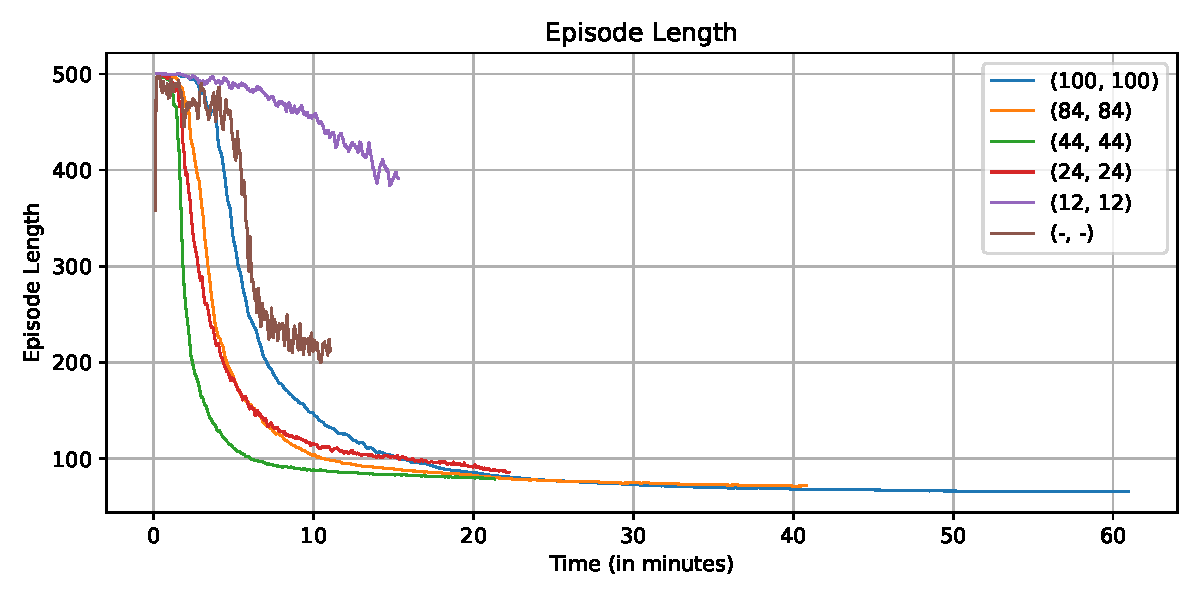
\includegraphics[clip, width=0.95\columnwidth]{figures/evaluation/observations/maze0318_ep_len_time.pdf}
    \end{center}
    \caption[Episode Length on the Corridor Environment using Different Observation Sizes]{Average episode length during training with different observation sizes on the corridor environment. The x-axis shows wall-clock time instead of steps to show effective performance.} \label{fig:ObsSize/Maze0318/EpLen}
\end{figure}


The results of our experiments can be found in Table \ref{tab:ObsSize}. We begin by looking at the results from the Corridor instance in Table \ref{tab:ObsSize} (a). We can see, that the agent is able to tolerate much lower observation sizes than 84 by 84. Even at a frame size of 24 by 24 (which is only about 8\% of the original input information) the agent is still able to solve the environment with only slightly worse performance. Interestingly the smaller frame size of 12 by 12 pixels is not sufficient to train the agent, while only a step counter as an observation is. We suspect that strong downscaling leads to many similar or even equal environment states even when particles are at very different locations, while the step counter input provides a clear distinction between states and therefore works better.

Different frame sizes do not only affect the performance of the learned strategy, but also have a great effect on wall-clock time. Figure \ref{fig:ObsSize/Maze0318/EpLen} shows the performance of the agents trained with different observation sizes in relation to time instead of steps. The time difference between input sizes does increase the larger the input gets. This is non surprising since the neural network needs to be larger and we therefore need to process more data. Due to hardware-related limitations this change in time is linear, but rather changes suddenly at certain points.

Let us now look at the results for the other instances in Table \ref{tab:ObsSize} (b) and (c). We can see, that even though the results were similar, there are some important differences: Even for slightly larger instances like the vessel instance, providing a larger input requires a change in network architecture to deal with the increased information. For both the vessel and the brain instance, increasing the observation size lead to much slower \textit{and} worse overall results. We will therefore try to improve the network to handle larger input sizes in Section \ref{sec:EvalNetworks}. Another important finding is, that we cannot simply downscale much larger instances and still expect good results. On the Brain instance the original 84 by 84 downscale was the tiniest observation size that still worked. This exposes a problem if we want to solve real-world instances which would be much larger or even three-dimensional. 


\subsection{Frame Stacking} \label{sec:Eval/FrameStack}
Frame stacking is important for settings where the agent must be able to estimate the movements of objects. For example if we want to drive a car and have top-down images of its position, we need to estimate its current velocity from its change of position, to calculate future movements. However in our particle environment, the movements of the particles will not be affected by past actions, since the particles do not have an internal velocity and stop after each move. We therefore expect frame stacking to only have a minor effect on the training process.   

\begin{table}[htp]
    \begin{center}
        \begin{tabular}{c}
            \begin{tabular}{rcrrrr}
                \toprule
                \multicolumn{1}{c}{Idx} & \multicolumn{1}{c}{Frame Stack} & \multicolumn{1}{c}{Best} & \multicolumn{1}{c}{Avg} & \multicolumn{1}{c}{Drop} & \multicolumn{1}{c}{Time}\\
                \midrule
                1 & 6 & 61.34 & 66.34 & 143k & 1:17:40h \\
                2 & 4 & 61.81 & 71.28 & 147k & 0:40:36h \\
                3 & 2 & 57.22 & 66.69 & 145k & 0:34:00h \\
                4 & 1 & \textbf{56.44} & \textbf{59.70} & \textbf{122k} & \textbf{0:31:25h} \\
                \bottomrule
            \end{tabular} \\
            \addlinespace[0.15cm]
            {\small (a) Results for the Corridor instance.} \\
            \addlinespace[0.5cm]
            \begin{tabular}{rcrrrr}
                \toprule
                \multicolumn{1}{c}{Idx} & \multicolumn{1}{c}{Frame Stack} & \multicolumn{1}{c}{Best} & \multicolumn{1}{c}{Avg} & \multicolumn{1}{c}{Drop} & \multicolumn{1}{c}{Time}\\
                \midrule
                1 & 6 & 107.91 & 108.86 & 569k & 2:02:54h \\
                2 & 4 & \textbf{91.06} & 96.72 & 532k & 1:10:00h \\
                3 & 2 & 92.06 & 99.84 & 443k & 0:59:14h \\
                4 & 1 & 93.16 & \textbf{94.32} & \textbf{382k} & \textbf{0:53:57h} \\
                \bottomrule
            \end{tabular} \\
            \addlinespace[0.15cm]
            {\small (b) Results for the Vessel Instance} \\
            \addlinespace[0.5cm]
            \begin{tabular}{rcrrrr}
                \toprule
                \multicolumn{1}{c}{Idx} & \multicolumn{1}{c}{Frame Stack} & \multicolumn{1}{c}{Best} & \multicolumn{1}{c}{Avg} & \multicolumn{1}{c}{Drop} & \multicolumn{1}{c}{Time}\\
                \midrule
                1 & 4 & \textbf{308.31} & \textbf{333.53} & 7.34M & 4:28:39h \\
                2 & 2 & 331.44 & 353.35 & 6.56M & 3:58:53h \\
                3 & 1 & 326.06 & 345.49 & \textbf{6.54M} & \textbf{3:49:05h} \\
                \bottomrule
            \end{tabular} \\
            \addlinespace[0.15cm]
            {\small (c) Results for the Brain Instance} \\
        \end{tabular}
        
    \end{center}
    \caption[Evaluation Results for Different Levels of Frame Stacking]{Results for different levels of frame stacking. The best values are marked in bold. We can see, that frame stacking does not improve learning for the basic maze environments. By disabling frame stacking (setting it to one) learning times can be significantly reduced (see (a)). Agents also learn better strategies on smaller instances using only single frames as input (see (a) bold). However this advantage does not seem to translate to larger instances (see (c)). We can argue, that the difference in performance is small enough, that the reduced training time compensates for the slightly worse performance. Without frame stacking, agents generally learn faster as they require both less steps (earlier drop time) and less computation time per step. The reduced computation time mainly originates from smaller neural networks due to the decreased input size. For (c) this difference is smaller, because the larger instance leads to a CPU instead of a GPU bottleneck.} \label{tab:Eval/FrameStacking}
\end{table}

We evaluated the effects of frame stacking on our three test instances and included the results  in Table \ref{tab:Eval/FrameStacking}. We can see, that our initial prediction was partially right and frame stacking does not seem to provide great benefits for training on our basic maze environments. Form Table \ref{tab:Eval/FrameStacking} (a) we can see, that removing frame stacking provides results in less overall time and also improves the final performance of the model for smaller instances. Unfortunately, this advantage seems to disappear for larger instances with longer training times (see Table \ref{tab:Eval/FrameStacking} (b) and (c)). By looking at Figure \ref{fig:Eval/FrameStacking/Maze0122} we can also see, that removing frame stacking may introduce more variance and training instability. 

Nevertheless, with less or no frame stacking we usually get comparably good results. Agents generally seem to learn faster, because the agent has to process and "understand" less information and therefore has to deal with less total states. As the agent does not need to know the position of particles over time, it can concentrate on the current position of the particles. The reduced input size also leads to smaller neural networks, which further accelerates learning in terms of wall-clock time. This can also be seen in Figure \ref{fig:Eval/FrameStacking/Maze0122} where we show the average episode length during training in relation to the training time. 

\begin{figure}[htp]
    \begin{center}
        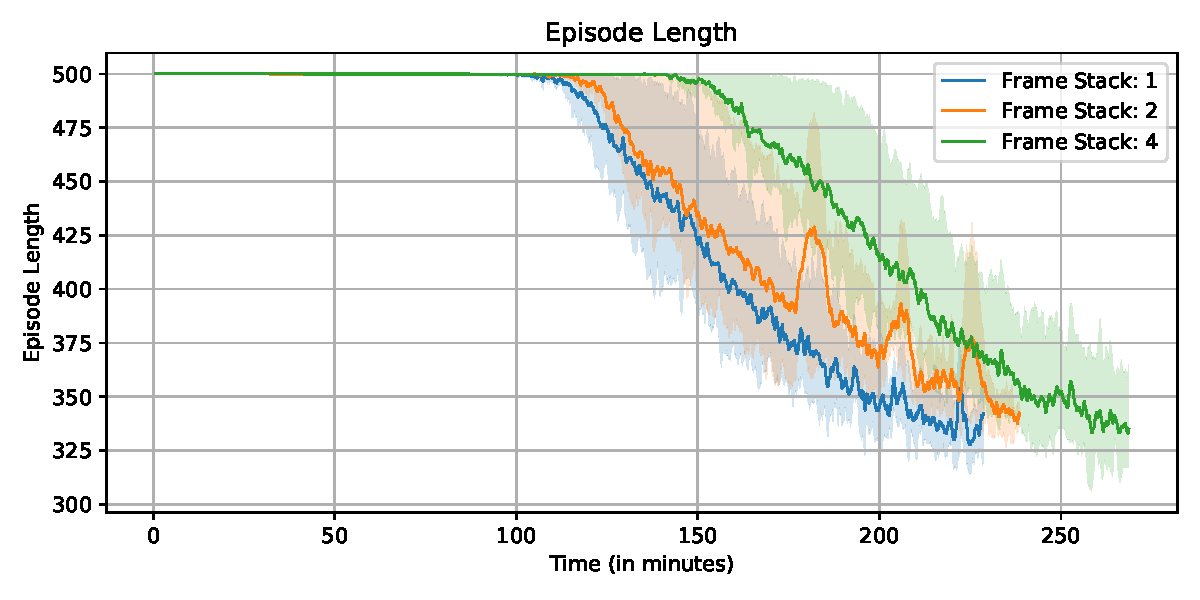
\includegraphics[clip, width=0.8\columnwidth]{figures/evaluation/observations/maze0122_frame_stack_ep_len.pdf}
    \end{center}
    \caption[Average Training Episode Length for Different Levels of Frame Stacking]{Average episode length during training for different levels of frame stacking. The x-axis shows wall-clock time for training sessions of 12 million steps. We can see, that less frame stacking improves learning speed, but introduces more training instability.} \label{fig:Eval/FrameStacking/Maze0122}
\end{figure}

\paragraph{Conclusion. } Following our results, when training agents for the simple maze environment, we can remove frame stacking without loosing any performance. However we have to be careful with this decision when extending or changing the setting. For noisy observations (see Section \ref{sec:EvalError}) as well as when dealing with particles which keep their velocity (see Section \ref{sec:EvalPhysical}) it might be a significant disadvantage to remove this information. 


\section{Network Architecture} \label{sec:EvalNetworks}
In this section we want to evaluate how much influence different network architecture has on the performance. For all past experiments we used the same neural network structure, using a simple CNN equal to the one used in previous experiments. In Section \ref{sec:Eval/NetworkStructure}, we will test other networks on our test instances, to see, if we can achieve an improvement in training time or final result by adding or removing layers. Finally, we will also evaluate if we are able to improve the performance, by replacing the leaky ReLU activation function in Section \ref{sec:Eval/ActivationFunctions}.

\subsection{Network Structure} \label{sec:Eval/NetworkStructure}
The CNN we used in past experiments consists of three convolutional layers with 32 ($8 \times 8, s=2$), 64 ($4\times4, s=2$) and 64 ($4 \times 4, s=1$) filters respectively, followed by a single fully connected layer with 512 neurons. The CNN extractor this network uses is used by many other authors who performed experiments on similar sized environments like the Atari game suite (e.g. \cite{burda2018large, burda2018exploration, mnih2015human}). We therefore expect the CNN to be fairly optimized for the given input and mostly focus on the structure of the fully connected layers. We also expect network sizes to only matter for larger, more complicated instances, where more complex behavior has to be learned. we therefore limit our tests to the Vessel and the Brain instance.

\begin{table}[htp]
    \begin{center}
        \begin{threeparttable}
            \begin{tabular}{rccrrrr}
                \toprule
                \multicolumn{1}{c}{Idx} & \multicolumn{1}{c}{CNN} & \multicolumn{1}{c}{MLP} & \multicolumn{1}{c}{Best} & \multicolumn{1}{c}{Avg} & \multicolumn{1}{c}{Drop} & \multicolumn{1}{c}{Time}\\
                \midrule
                1 & default & [512] & \textbf{91.06} & \textbf{96.72} & 532k & 1:10:00h \\
                2 & default & [512, {'pi': [512], 'vf': [512]}] & 101.03 & 104.18 & 538k & 1:10:47h \\
                3 & default & [512, 512] & 95.97 & 99.09 & 508k & 1:10:34h \\
                4 & default & [256] & 94.16 & 98.81 & 506k & \textbf{1:09:27h} \\
                5 & default & [256, 448, {'pi': [448], 'vf': [448]}] & 98.38 & 107.02 & 536k & 1:10:37h \\
                6 & default & [128] & 101.97 & 104.03 & 476k & 1:09:56h \\
                7\tnote{1} & modified\tnote{2} & [512] & 110.00 & 114.35 & \textbf{413k} & 1:51:27h \\
                \bottomrule
            \end{tabular}
            \begin{tablenotes} \footnotesize
                \item[1] We removed downscaling for this experiment.
                \item[2] Structure: ('conv', 32, 8, 4), ('pool', 2, 2), ('conv', 64, 4, 2), ('conv', 64, 3, 1)
            \end{tablenotes}

        \end{threeparttable}
        
    \end{center}
    \caption{Vessel}
\end{table}

\begin{table}[htp]
    \begin{center}
        \begin{threeparttable}
            \begin{tabular}{rccrrrr}
                \toprule
                \multicolumn{1}{c}{Idx} & \multicolumn{1}{c}{CNN} & \multicolumn{1}{c}{MLP} & \multicolumn{1}{c}{Best} & \multicolumn{1}{c}{Avg} & \multicolumn{1}{c}{Drop} & \multicolumn{1}{c}{Time}\\
                \midrule
                1 & default & [512] & \textbf{308.31} & 333.53 & 7.34M & 4:28:39h \\
                2 & default & [512, {'pi': [512], 'vf': [512]}] & 317.84 & 334.83 & \textbf{6.79M} & \textbf{4:24:58h} \\
                3\tnote{1} \ \tnote{2} & modified\tnote{3} & [512] & 326.53 & \textbf{326.53}\tnote{2} & 7.41M & 16:08:57h \\
                \bottomrule
            \end{tabular}
            \begin{tablenotes} \footnotesize
                \item[1] We changed downscaling to ($168 \times 168$) for this experiment.
                \item[2] Due to the increase in training time, this experiment does not use multiple trials. 
                \item[3] Structure: ('conv', 32, 8, 4), ('pool', 2, 2), ('conv', 64, 4, 2), ('conv', 64, 3, 1)
            \end{tablenotes}
        \end{threeparttable}
    \end{center}
    \caption{Brain}
\end{table}

Table TODO, shows the results on the Vessel instance.


\subsection{Activation Functions} \label{sec:Eval/ActivationFunctions}

\begin{table}[htp]
    \begin{center}
        \begin{tabular}{rccccrrrr}
            \toprule
             &  &  &  &  & \multicolumn{2}{c}{Episode Length} & \\
            \cmidrule(lr){6-7}
            \multicolumn{1}{c}{Idx} & \multicolumn{1}{c}{CNN} & \multicolumn{1}{c}{MLP} & \multicolumn{1}{c}{CNN Act} & \multicolumn{1}{c}{MLP Act} & \multicolumn{1}{c}{Best} & \multicolumn{1}{c}{Avg} & \multicolumn{1}{c}{Drop} & \multicolumn{1}{c}{Time}\\
            \midrule
            1 & default & [512] & selu & selu & \textbf{54.50} & \textbf{55.88} & 184k & 0:44:21h \\
            2 & default & [512] & Leaky ReLU & tanh & 58.06 & 69.75 & \textbf{146k} & \textbf{0:40:24h} \\
            3 & default & [512] & Leaky ReLU & Leaky ReLU & 61.81 & 71.28 & 147k & 0:40:36h \\
            \bottomrule
        \end{tabular}
    \end{center}
    \caption{Activations - Maze0318}
\end{table}

\begin{table}[htp]
    \begin{center}
        \begin{tabular}{rccccrrrr}
            \toprule
             &  &  &  &  & \multicolumn{2}{c}{Episode Length} & \\
            \cmidrule(lr){6-7}
            \multicolumn{1}{c}{Idx} & \multicolumn{1}{c}{CNN} & \multicolumn{1}{c}{MLP} & \multicolumn{1}{c}{CNN Act} & \multicolumn{1}{c}{MLP Act} & \multicolumn{1}{c}{Best} & \multicolumn{1}{c}{Avg} & \multicolumn{1}{c}{Drop} & \multicolumn{1}{c}{Time}\\
            \midrule
            1 & default & [512] & selu & selu & 96.71 & 97.27 & 505k & 1:19:05h \\
            2 & default & [512] & Leaky ReLU & tanh & 99.94 & 102.25 & \textbf{475k} & 1:10:54h \\
            3 & default & [512] & Leaky ReLU & Leaky ReLU & \textbf{91.06} & \textbf{96.72} & 532k & \textbf{1:10:00h} \\
            \bottomrule
        \end{tabular}
    \end{center}
    \caption{Activations - Vessel}
\end{table}


\begin{table}[htp]
    \begin{center}
        \begin{tabular}{rccccrrrr}
            \toprule
            \multicolumn{1}{c}{Idx} & \multicolumn{1}{c}{CNN} & \multicolumn{1}{c}{MLP} & \multicolumn{1}{c}{CNN Act} & \multicolumn{1}{c}{MLP Act} & \multicolumn{1}{c}{Best} & \multicolumn{1}{c}{Avg} & \multicolumn{1}{c}{Drop} & \multicolumn{1}{c}{Time}\\
            \midrule
            1 & default & [512] & selu & selu & 311.84 & \textbf{328.06} & \textbf{5.94M} & 4:39:51h \\
            2 & default & [512] & Leaky ReLU & tanh & 401.34 & 415.33 & 9.68M & \textbf{4:24:44h} \\
            3 & default & [512] & Leaky ReLU & Leaky ReLU & \textbf{308.31} & 333.53 & 7.34M & 4:28:39h \\
            \bottomrule
        \end{tabular}
    \end{center}
    \caption{Activations - Brain}
\end{table}


\section{Extended Environment Models} \label{sec:EvalExtendedModels}
Extended Environment Models
\subsection{Dealing with Error} \label{sec:EvalError}
Dealing with Error
\subsection{Physical Particles} \label{sec:EvalPhysical}
Physical Particles
\section{Randomized Instances} \label{sec:EvalRandomness}
Randomized Instances
\subsection{Random Goal Positions} \label{sec:EvalRandomGoals}
Random Goal Positions
\subsection{Random Mazes} \label{sec:EvalRandomMaze}
Random Mazes
\section{Comparison to Algorithmic Approaches} \label{sec:EvalAlgorithms}
Comparison to Algorithmic Approaches